\documentclass[11pt,a4paper,oldfontcommands]{memoir}
\usepackage[utf8]{inputenc}
\usepackage[T1]{fontenc}
\usepackage{microtype}
\usepackage[dvips]{graphicx}
\usepackage{xcolor}
\usepackage{times}

\usepackage[
breaklinks=true,colorlinks=true,
%linkcolor=blue,urlcolor=blue,citecolor=blue,% PDF VIEW
linkcolor=black,urlcolor=black,citecolor=black,% PRINT
bookmarks=true,bookmarksopenlevel=2]{hyperref}

\usepackage{geometry}
\usepackage{amsmath}
\DeclareMathOperator*{\argmin}{argmin}
\DeclareMathOperator*{\argmax}{argmax}

\usepackage{caption}
\usepackage{algorithm}
\usepackage{algpseudocode}

% PDF VIEW
% \geometry{total={210mm,297mm},
% left=25mm,right=25mm,%
% bindingoffset=0mm, top=25mm,bottom=25mm}
% PRINT
\geometry{total={210mm,297mm},
left=20mm,right=20mm,
bindingoffset=10mm, top=25mm,bottom=25mm}

\OnehalfSpacing
%\linespread{1.3}

%%% CHAPTER'S STYLE
%\chapterstyle{bianchi}
\chapterstyle{ger}
%\chapterstyle{madsen}
%\chapterstyle{ell}
%%% STYLE OF SECTIONS, SUBSECTIONS, AND SUBSUBSECTIONS
\setsecheadstyle{\Large\bfseries\sffamily\raggedright}
\setsubsecheadstyle{\large\bfseries\sffamily\raggedright}
\setsubsubsecheadstyle{\bfseries\sffamily\raggedright}


%%% STYLE OF PAGES NUMBERING
%\pagestyle{companion}\nouppercaseheads 
%\pagestyle{headings}
%\pagestyle{Ruled}
\pagestyle{plain}
\makepagestyle{plain}
\makeevenfoot{plain}{\thepage}{}{}
\makeoddfoot{plain}{}{}{\thepage}
\makeevenhead{plain}{}{}{}
\makeoddhead{plain}{}{}{}


\maxsecnumdepth{subsection} % chapters, sections, and subsections are numbered
\maxtocdepth{subsection} % chapters, sections, and subsections are in the Table of Contents


%%%---%%%---%%%---%%%---%%%---%%%---%%%---%%%---%%%---%%%---%%%---%%%---%%%

\begin{document}

%%%---%%%---%%%---%%%---%%%---%%%---%%%---%%%---%%%---%%%---%%%---%%%---%%%
%   TITLEPAGE
%
%   due to variety of titlepage schemes it is probably better to make titlepage manually
%
%%%---%%%---%%%---%%%---%%%---%%%---%%%---%%%---%%%---%%%---%%%---%%%---%%%
\thispagestyle{empty}

{%%%
\sffamily
\centering
\Large

~\vspace{\fill}

{\huge 
An Optimization for Convolutional Network Layers using the Viola-Jones Framework and Ternary Weight Networks
}

\vspace{2.5cm}

{\LARGE
Rhys Agombar
}

\vspace{3.5cm}

A thesis submitted in partial fulfillment for the\\
degree of Master of Science\\[1em]
in the\\[1em]
Faculty of Computer Science\\
Rheinische Friedrich-Wilhelms-Universität Bonn

\vspace{3.5cm}

Supervisors: Prof. Dr. Christian Bauckhage, Prof. Dr. Stefan Wrobel \\
Advisor: Dr. Rafet Sifa

\vspace{\fill}

October 2020
%%%
}%%%

\cleardoublepage%%%---%%%---%%%---%---%%%---%%%---%%%---%%%---%%%---%%%---%%%---%%%---%%%
%%%---%%%---%%%---%%%---%%%---%%%---%%%---%%%---%%%---%%%---%%%---%%%---%%%
\tableofcontents*

%\clearpage%---%%%---%%%---%%%---%%%---%%%---%%%---%%%---%%%---%%%---%%%---%%%---%%%
%%%---%%%---%%%---%%%---%%%---%%---%%%---%%%---%%%---%%%---%%%---%%%---%%%

\chapter{Introduction}
How can we get a computer to see the world the way a human does? This is a question that has perplexed researchers for decades. Since as early as 1966 \cite{mit_cv}, where a group of students were assigned a summer project to detect object and background areas in an image, attempts have been made to solve this, with varying degrees of success. Given that, over fifty years later, we are still working on it, clearly the complexity of the problem was underestimated. Despite its difficulty, this field, computer vision, has a myriad of applications, leading to the continued investment of time and money into ongoing research. From semi-autonomous vehicles to medical imaging systems, to facial filters for social media apps, the fruits of these labours can be seen around us in the world today. Despite these successes, though, the field still has problems left to solve.

Originally, the problem was just getting the systems to work accurately. In the beginning days of computer vision, hand-crafted features for classifiers, complex mathematical algorithms, or basic image templates were used to try and classify images or locate objects in a scene. These had some success, but encountered difficulties when attempting to generalize. Custom classifiers designed to detect upright, forward facing faces tended to perform poorly when the faces were rotated or viewed from the side, for example, and though these algorithms were usually fairly light weight and quick, failing quickly does not constitute a success. This limited their deployments to use cases where specific assumptions could be made. Going back to our face detection example, this might be something like automatically focusing a camera based on detected faces in the frame, since one would assume that the subjects of the picture would be facing the camera more often than not. 

With the advent of artificial neural networks and, more importantly, their extension of convolutional neural networks, however, this problem began to disappear. Neural networks are very flexible when it comes to their learning and classification, provided they are given a good architecture and sufficient data to be trained, and convolutional networks (which take advantage of local data correlations), are even more so. Indeed, modern architectures, such as the one proposed by Touvron \textit{et al.} \cite{fix}, are beginning to approach the levels of human error recorded by the ImageNet (a popular, large-scale image dataset) visual recognition challenge paper \cite{VGG16_challenge}. Unfortunately, the downside of these powerful networks is that they tend to be very large or take a long time to compute, which makes them impractical for applications that require real-time performance. 

Making accurate classifications is well and good, but trying to make accurate classifications \textit{fast} is an entirely different beast. For things like self-driving cars, the system cannot afford to wait five, ten, or fifteen seconds to determine if the object it's about to run over is a harmless leaf or a human child. By the time it arrives at its answer, it will already be too late. As such, a significant amount of research is now being done to create solutions to this problem that can trade off ever-smaller amounts of accuracy for ever-greater gains in speed. The optimization we propose in this thesis is one of these solutions. 

As mentioned before, classical computer vision algorithms tend to be relatively light weight, and in particular, the Viola-Jones Object Detection Framework \cite{viola} is capable of detecting objects like faces extremely quickly, even on weak hardware. The two of the ways it achieves this are through using an optimized representation of an image, called an integral image, and using special classification features that have been designed to take advantage of the new representation, allowing for rapid computation. Unfortunately, while quick at detecting faces in an image, it runs into the same problems of not being very generalizable, and struggling with rotated or side-viewed faces. This is the opposite problem that neural networks have, which are accurate and highly generalizable, but slow. Is there a way to combine the speed of the Viola-Jones framework with the accuracy of artificial neural nets? This is the question this thesis was inspired by.

Our contribution is a combination of these two methods. Taking inspiration from the the Viola-Jones framework, we train a convolutional neural network, but restrict the weights to ternary values ($-1$, 0, and $+1$), as they are the same values that the framework uses in its classification features. We then use these trained weights to define a set of custom filters composed of rectangular positive and negative regions, similarly to how the features from Viola-Jones are defined. Lastly, we change the structure of our input data. Rather than sending the network standard images, we instead convert them to integral images as that is the data structure rectangular features are able to be computed for with maximum efficiency. By combining the general feature structure and integral images from the Viola-Jones framework with powerful ternary-weighted neural networks, we are capable of accelerating the first layer of a network with little to no cost to the network's overall accuracy. When evaluated on the MNIST \cite{mnist} and CIFAR-10 \cite{cifar} datasets, we see that our method produces accuracies within approximately half a percentage point of their respective reference networks, while using only $~64\%$ of the total number of operations required to compute the first $5\times5$ convolutional layer. Before we can get into discussing the details of our method and experiments, however, we first must go over the recent literature about optimizing neural network performance, as well as the background theory for why it works. 


\chapter{Literature Review}

The problem of improving neural network performance is not a new one. For years, scientists have been working to create faster and more efficient networks without sacrificing too much in the way of accuracy. Of course, convolutional neural networks require different optimization strategies than standard neural nets, due to their differing architecture, however, their popularity means they have still attracted significant amounts of research. This research can be broadly categorized into four different categories: optimizing filter representations, filter or weight pruning, mathematical optimizations, and architectural optimizations. In this chapter, we will go over some of the most recent papers from each of these, and at the end, discuss what makes this thesis unique with regards to them. 

\section{Optimized Filter Representations}
Filter optimizations are one of the ways that convolutional networks can be sped up, the idea behind them being that if the values of the filters can be computed quickly, the performance of the network will improve as well. Compared to the other categories mentioned before, there has been relatively little research conducted on this topic, with only a couple of recent papers being found.

%"Learning Versatile Filters for Efficient Convolutional Neural Networks"
We begin this section by discussing Wang \textit{et al}'s paper \cite{Versatile}. In it, the authors attempt to speed up convolutional networks by proposing more efficient filters they call `versatile filters'. These are a set of secondary filters constructed from the primary filters, using a series of pre-defined rules. These secondary filters inherit the weights of their parent filters and can be computed simultaneously, but have different receptive fields and produce different feature values. This allows the number of filters in a given layer to be lower without sacrificing accuracy, thus reducing the overall number of FLOPs (floating point operations) required and therefore speeding up the network. 

%"Rethinking Depthwise Separable Convolutions:How Intra-Kernel Correlations Lead to Improved MobileNets"
Our second paper, Hasse \textit{et al.}, \cite{Depthwise} proposes a new type of convolutional layer, called Blueprint Separable Convolutions (BSConv). BSConvs exploit high levels of redundancy along a CNN's depth axis by representing filter kernels using a single 2d blueprint distributed along the depth axis. These can be used as direct replacements for convolutional layers, and reduce the number of parameters in the network, improving performance and efficiency.

% Deep Neural Networks with Box Convolutions
Lastly, Burkov \textit{et al.} \cite{BoxConv} changed their network such that it now learns rectangular box filters instead of regular ones. In their network, only the dimensions and spatial offsets of the boxes are learned, and the average value of the filter will be returned as the filter response. The values for this are computed using integral images, which are optimized data structures for summing image values over a rectangular area. The combination of the low number of parameters for each filter, along with the use of integral images, creates a very efficient and quick neural network that maintains high levels of accuracy.

\section{Pruning}
Compared to optimizing filters, pruning connections or whole filters is a much more popular approach to optimization. This involves removing the less useful parts of a network to decrease the number of operations needed to process it, increasing speed while decreasing the network's size. Since the components removed tend to be of only marginal use, the overall accuracy of a system does not usually suffer significantly. In this section, we'll list some of the most recent attempts at this, beginning with He \textit{et al}.

% Learning Filter Pruning Criteriafor Deep Convolutional Neural Networks Acceleration
He \textit{et al.} \cite{PruningC} published two different papers on this topic, recently. The first proposes a differentiable pruning criteria sampler (a method called Learning Filter Pruning Criteria, or LFPC) which, as the name suggests, allows the network to learn the criteria it will use for pruning itself. This is optimized by the validation loss of the pruned networks. Other papers have proposed similar systems, but this one is different because it adaptively selects different criteria for each layer (allowing it to handle different filter distributions), and considers the contribution of all layers rather than looking at each layer individually. This system allows for highly effective pruning of the network.

% Filter Pruning via Geometric Medianfor Deep Convolutional Neural Networks Acceleration
The second paper by He \textit{et al.} \cite{PruningG} proposes a method of pruning the network's filters using the geometric median. This method is unique in that rather than pruning the filters with the lowest contribution, their method prunes the most replaceable filters instead. Since the network retains other filters similar to the ones being pruned, this allows for it to maintain its abilities to handle a diverse set of inputs, resulting in only a slight decrease in accuracy.

% HRank: Filter Pruning using High-Rank Feature Map
Moving on to other authors, in Lin \textit{et al.}'s paper \cite{HRank}, the authors observed that the average rank of feature maps generated by a filter was always the same, regardless of input. Using this, their pruning method determined which filters would produce lower ranked feature maps, and removed them. Since feature maps with a low rank contain less information than those with a high rank, pruning the corresponding filters allowed for a large reduction in the required number of FLOPs, leading to gains in performance with little loss of accuracy.

% Dynamic Channel Pruning: Feature Boosting and Suppression
Gao \textit{et al.} \cite{DCPruning} proposed a method of pruning called `Feature Boosting and Suppression (FBS)', which was inspired by the observation that the importance of the learned filters at a given time will vary depending on the instance of the input data being processed. Their method allows for the amplification of the most important convolutional channels at run time, and for the network to skip unimportant ones. As part of this, they add some light-weight auxiliary connections to the convolutional layer, which predict which features are important or not. By skipping rather than truly pruning portions of the network, the entire network is preserved, allowing it retain its full capabilities while also improving efficiency and speed. 

% Gate Decorator: Global Filter Pruning Method for Accelerating Deep Convolutional Neural Networks
You \textit{et al.} \cite{GateD} introduce an algorithm for global filter pruning called `Gate Decorator'. In this, they multiply the output of standard convolutional layers by channel-wise scaling factors, and use Taylor expansion to estimate the changes that would occur in the loss by setting certain scaling factors to 0 (equivalent to removing the filter). These estimations are then used to determine the importance rankings of each filter in the network, and the least important ones will be pruned. They also propose two iterative frameworks for repeated pruning.

% Learning both Weights and Connections for Efficient Neural Network
The final pruning paper, Han \textit{et al.} \cite{LWC}, details a 3-step method of pruning redundant network connections. The network is first trained to determine which connections are the most important. It is then pruned, with the connections whose weights are lower than a given threshold being deleted. In the last step, it is retrained to attain the final weights of the remaining sparse connections. This process can then be repeated to further reduce the number of network connections.

\section{Mathematical Optimizations}
From filtering algorithms to reparameterization tricks, optimizing the math running a convolutional network is another popular area of research, rivaling that of pruning. The methods from this section promise significant speedups, some of them without cost, and on one occasion, with an increase in accuracy - a phenomenon unheard of in the pruning section. 

% Compression of Deep Convolutional Neural Networks for Fast and Low Power Mobile Applications
The first paper we discuss is Kim \textit{et al.} \cite{FLMA}, which proposes a scheme to compress a convolutional network to improve its runtime and reduce its model size and energy consumption. The intention of this was to allow the use of convolutional nets on low-power mobile devices. This scheme consists of three steps: rank selection using variational Bayesian matrix factorization, low-rank tensor decomposition using Tucker decomposition on the kernel tensor, and a final, fine-tuning step. In their evaluation, the authors show that they managed to achieve their goals with only a small loss of accuracy.

% Speeding up Convolutional Neural Networkswith Low Rank Expansions
The method from Jaderberg \textit{et al.}'s paper \cite{LRE} exploits cross-channel and filter redundancy to speed up computations by constructing new low-rank basis filters that are rank-1 in the spatial domain. These filters are not true convolutional filters, rather they are an approximation that is much quicker to compute. The main contributions of this paper are its two different approximation schemes for constructing these, as well as two different optimization methods to ensure good performance. 

% Faster Neural Networks Straight from JPEG
Gueguen \textit{et al.} \cite{FJPEG} modify the data being fed to the network, as well as the network architecture to accommodate for the new input shapes. In this paper, instead of training and testing their network with JPEG images, the authors use the `blockwise discrete cosign transform' coefficients computed in the middle of the JPEG codec, which represent partly decoded images. Once the network was redesigned to accommodate these, the authors found that it resulted in both a quicker and more accurate network.

% Efficient Sparse-Winograd Convolutional Neural Networks
Liu \textit{et al.}'s paper \cite{Winograd} proposes a modification to Winograd's minimal filtering algorithm, which is a method of reducing the number of multiplications needed to perform $3 \times 3$ kernel convolutions. This method is incapable of using pruning to exploit sparsity, however, because the Winograd algorithm fills in the 0s in the weight and feature values, thus eliminating the gains that can be made by exploiting sparsity. In this paper, the authors found that by moving the activation functions of their network layers to after the Winograd transform, and pruning the weights after the transform instead of before, the two methods can be used together to allow for large reductions in the number of needed multiplications. This allows for a much faster network, with less than a 0.1\% loss in accuracy.  

% PerforatedCNNs: Acceleration through Elimination of Redundant Convolutions
In Figurnov \textit{et al.} \cite{PerfCNN}, the authors introduce perforated convolutional networks, which were inspired by the loop perforation techniques used in source code optimization. Their approach is one that exploits spatial redundancy using the interpolation of filter responses to increase the speed of their network. For this, they use perforation masks, which define a subset of positions in the output to be evaluated, and then use interpolation to estimate the values between them. The paper contributes a set of different approaches to select these perforation masks, and a method of choosing different combinations of masks for different layers.

% Binary Weight Networks
Rastegari \textit{et al.} \cite{binary} propose the use of binary weights in their neural networks to increase the speed of operations and decrease model size. The use of these weights means that the mathematical operations in a convolutional network are capable of being expressed entirely through additions and subtractions, which are less computationally expensive to compute. In this paper, the authors propose methods for converting full precision weights to these binary weights, as well as a network architecture called `XNOR-nets'. This architecture extends these efficiency gains even further, by using XNOR and bit-counting operations to produce massive speedups.

% Ternary Weight Networks
Li \textit{et al.}'s paper \cite{ternary} is an extension of the previously mentioned binary weight networks. Using binary weights results in fast performance, but has a significant accuracy cost. By changing these weights to ternary weights (spanning the range of $-1$, 0, and $+1$), the network's learning capabilities can be increased while maintaining the same gains in efficiency produced by the original binary weights. This makes the speed-accuracy trade-off more palatable. 

% LEARNINGDISCRETEWEIGHTSUSING   THELOCALREPARAMETERIZATIONTRICK
The last paper in this section, Shayer \textit{et al.} \cite{Reparam}, is yet another extension, this time for the ternary networks, as well as the binary ones, mentioned in the last two paragraphs. In this, they iterate upon the existing efficiency improvements from the prior papers by introducing LR-nets (local reparameterization networks). These decrease the loss of accuracy binary and ternary nets produce, compared to their full-precision networks. LR-nets allow for a new method of training networks containing discrete weights, using stochastic parameters and the local reparameterization trick. While this does not improve the speed of a network, the authors' contribution improves the accuracy of the system, again, making the speed-accuracy tradeoff even more palatable.

\section{Architectural Optimizations}
The last method of optimization we'll go over is changing the architecture of the networks to be more efficient. By altering the design of layer archetypes, their connections, or by simply rearranging the network's layers, architectural optimizations can lead to improved performance. 

% ChannelNets: Compact and Efficient ConvolutionalNeural Networks via Channel-Wise Convolutions
Gao \textit{et al.} \cite{ChannelNet} is a paper that modifies the convolutional layers of a network by replacing them with more compact and efficient channel-wise convolutions, resulting in lighter weight architectures the authors call `ChannelNets'. Their contributions are the development of channel-wise convolutions, depth-wise separable channel-wise convolutions, and a convolutional layer for classification. These layers and methods are sparser than normal convolutional architectures, which allow for faster execution.

% Dynamic Convolutions: Exploiting Spatial Sparsity for Faster Inference
Verelst \textit{et al.} \cite{DynaConv} exploit the fact that convolutions perform the same operations on every pixel in the image, which can be inefficient. They instead propose dynamically applying convolutions to the image by adding a residual block to the network architecture. In this block, a gating branch learns which positions in the image the convolutions should be computed for, allowing for unimportant parts of the image to be ignored, thus reducing the amount of processing needed. 

%- Convolutions perform same operations on every pixel in the image (inefficient)
%- propose dynamically applying convolutions to image
%- residual block where small gating branch learns which spatial positions should be evaluated (For each residual block,a small gating network chooses the locations to apply dy-namic convolutions on)
%- gating network decisions are trained using Gumbel-Softmax trick

% ShuffleNet: An Extremely Efficient Convolutional Neural Network for MobileDevices
In Zhang \textit{et al.} \cite{Shuffle}, the authors propose a highly efficient convolutional neural net architecture, named `ShuffleNet'. In this, they utilize two new operations, pointwise group convolution and channel shuffling. Pointwise group convolutions help to reduce the complexity of $1\times1$ convolutions, and channel shuffling helps information to flow between feature channels in the network. This network design runs approximately 13$\times$ faster than AlexNet \cite{alex}, while maintaining similar accuracy.

% Densely Connected Convolutional Networks
Huang \textit{et al.} \cite{DCConv} propose an architecture called DenseNet, which is a dense convolutional network. In this, every layer in the network is connected to every other layer in a feed-forward fashion. One of the benefits of these dense connections is that the network no longer needs to learn redundant filters, which means layers can be defined to be very narrow, with comparatively few filters in each of them. This leads to an overall reduction in the number of parameters, allowing for faster inference, but at the same time, maintains high levels of accuracy. 

% LCNN: Lookup-based Convolutional Neural Network
A lookup-based convolutional network, published in Bagherinezhad \textit{et al.} \cite{LCNN}, introduces an architecture where the convolutions are encoded into a dictionary. This architecture is trained to learn a dictionary that covers the space of the weights in the convolutional network, as well as a small number of linear combinations. Because dictionary lookups are very fast, this network experiences a significant speedup when using them, while still performing accurately.

%SaccadeNet: A Fast and Accurate Object Detector
Lan \textit{et al.}'s paper \cite{Sacc} is the final one we will go over. It details an architecture for object detection, inspired by human eye saccades. This consists of four parts: the center attentive module, which predicts an object's center location as well as its category, the attention transitive module, which is used to predict rough locations of bounding box corners that will encompass the object, the corner attentive module, which encourages the backbone of the network to pay more attention to the object's boundaries, and the aggregation attentive module, which uses the features from the center and corner points to refine the bounding boxes. This network's architecture is capable at running in real-time, processing 28 frames per second when configured for maximum accuracy, and 118 frames per second when the required accuracy is lower. 

% Fast Sparse ConvNets
%Elsen \textit{et al.} \cite{FSConv} introduces a family of efficient, sparse kernels for `sparse matrix-dense matrix multiplication', specifically designed to speed up sparse neural networks  convolutional neural nets. 
%- efficient versions of sparse primitives (like convolution)

% Accelerating Convolutional Neural Networks via Activation Map Compression --- Actually Math?
%Our final paper, by Georgiadis \cite{AccConv}, proposes a three-stage compression and acceleration pipeline that sparsifies, quantizes and entropy encodes the activation maps of convolutional neural networks. 

%- Sparsification leads to increased representative power of activation maps
%- Quantization and Entropy Encoding the sparser activation maps leads to higher compression. 
%- Sparsification increases speed, Quant and Entropy increase compression

\section{Justification of Our Work}
With so many different approaches to optimizing convolutional networks, we need to justify why our method is relevant and different from the others. Our method does not prune weights or filters to achieve its speedup, despite this approach's popularity, and does not alter the network architecture enough to be considered an architectural optimization. Instead, it is a unique combination of existing filter and mathematical optimizations to achieve further efficiency gains. Like Burkov \textit{et al.} \cite{BoxConv}, we use integral images to speed up the computation of filter values, and like Li \textit{et al.} \cite{ternary}, we use ternary weights to optimize the network, however, to the best of our knowledge, these two approaches have never been combined before. Additionally, as per the original paper detailing the Viola-Jones Object Detection Framework \cite{viola}, our filters are more expressive than Burkov \textit{et al.}'s, as they each learn arrangements of four different rectangles rather than a single box's location and dimensions. Because of this unique combination of methods and modifications, our contribution exists within a space that has, until now, never been explored, making the work sufficiently novel to justify its existence. Our results also show good performance gains with minimal losses of accuracy when compared to standard ternary networks, so if nothing else, it exists as a useful iteration upon these ideas. 

% ECA-Net: Efficient Channel Attention for Deep Convolutional Neural Networks
%Wang \textit{et al.} \cite{ECA}
%- uses channel attention
%- Propose Efficient Channel Attention (ECA) module
%- Only involves a handful of parameters, which brings performance gains
%- Speeds up channel attention stuff specifically
%From different paper:
%- Channel of feature map is considered to be feature detector
%- Channel attention focuses on what is meaningful given an input image
%- "We produce a channel attention map by exploiting the inter-channel relationship of features."


% Big-Little Net: An Efficient Multi-Scale Feature Representation for Visual and Speech Recognition
%Chen \textit{et al.} \cite{BLN}
%- Proposes efficient network architecture. 
%- Multipbranch network with different computational complexities at different branches with different resolutions
%- Frequent merging of features from branches obtains multi-scale features while using less computation
%- Significant computational savings

% If we need it, add the FRCNN, Faster RCNN and YOLO networks to this, but they're pure architecture


\chapter{Background}
Before we can go into describing our proposed solution in detail, we need to go over some background information to provide an understanding of how we got to this point, and why our network works the way it does. First, we'll go over some general image processing concepts, followed by detailing the Viola-Jones Object Detection Framework, neural networks (in general, and as they pertain to this thesis), commonly used datasets, and finally, our motivation for using the particular methods we proposed.

\section{Image Processing}
Image processing, as the name suggests, involves passing images through mathematical algorithms to produce desirable outputs based on the input data. For example, these outputs could be higher quality versions of the original image, in the cases of upscaling or denoising, or non-image outputs, like bounding boxes for image segmentation or single values for image classification. In this thesis, we'll focus on the example of image classification, as it is the most relevant topic to our work and the experiments we conducted.

The methods used for image classification have, historically, relied on hand crafted algorithms or statistical models for computing their outputs, though modern approaches using artificial neural networks have become massively more popular over the years. This thesis is mostly about the latter approach, and as such, we will not go into much detail about classical methods aside from one, the Viola-Jones Object Detection Framework, since parts of it are directly used by this thesis. In order to discuss these methods, though, we first need to go over two foundational ideas: Features and Feature Maps.

\subsection{Features}
One of the problems encountered when trying to classify or process images is the question of what sort of data should be used for the classification functions. Let us take the example of trying to detect faces in an image, since this is the same use case the Viola-Jones Object Detection Framework was designed for. Given a section of the image containing a face, how would one identify it as such? A human looking at it might point to the eyes and nose, or possibly the contours of the chin or hair, as evidence that it is a face, but how would one define these in terms that a computer would understand? As is, the only thing that the computer sees is an array of colour values for each pixel. These are problematic because each pixel contains very little information, individually. Though one could devise sets of rules for classifying based on the pixel colours at certain locations, things like shadows, noise, and the natural diversity of facial structures would all confound this. As such, a different way of expressing the data is needed.

The new representation is called a 'Feature'. In the context of image classification, rather than containing only a single pixel's colour value, features can specify structures in the data providing more useful information about it overall. They can also be used to encode expert knowledge that would be difficult for an automatic system to learn on its own. These could be things like the edge or corner points in an image, or, in the case of the Viola-Jones Framework, regions representing the relationship between light and dark areas. Observe the example given in Figure \ref{fig:vj_feature_example}. Note how, on the face, the pixels on the eyes are darker than the surrounding pixels. This is a general pattern that occurs on many people's faces, so features can be used to represent it. In the middle images, a feature constructed from two horizontal rectangles is used to represent the light cheek-bones appearing below the dark eyes, and likewise, the right-most images contain a feature representing the contrasts between the eyes and the nose-bridge. Classifications can then be made based on the presence and strength of features like these, allowing the creation of highly accurate detection and classification systems that perform much better than those operating on individual pixel values. Because of this, features are found in almost all intelligent systems, from statistical models to neural nets, and from them, feature maps can be computed.

\begin{figure}
    \centering
    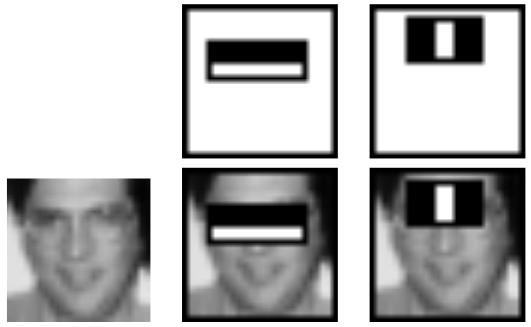
\includegraphics[height=15em]{Images/vj_feature_example.png}
    \caption{An example of two different Haar-like features used in the Viola-Jones Framework (taken from \cite{viola}). In the middle images, the relationship between the bright cheek-bones and dark eyes are represented, and in the right-most image, the contrast between the nose-bridge and the eyes is captured.}
    \label{fig:vj_feature_example}
\end{figure}

\subsection{Feature Maps}
Feature maps are commonly used in problems like image classification or segmentation. These are data structures, often similar to images, that describe the presence (or lack therefore) of a given feature at different points of the input image. Let us take the process of template matching as an example. Suppose we had an image of a scene and an image of a face, and wished to use the face to determine the presence of a certain person within the scene. In this case, the face would be the feature acting as a data representation of the person. By sliding the face image across the scene image and comparing the differences between the two images at each individual position, a feature map can be created. This map would contain a set of values quantifying the amount of difference at each point, showing locations where the feature responded strongly. Areas in this map with a very low `difference' would show a high feature response and correspond to locations where the face is present. An example of this is shown in Figure \ref{fig:template_matching}. For systems like convolutional neural nets, this type of data representation is extremely useful. In these networks, rather than a pre-defined image being used as the feature, each layer of the network learns its own features dynamically, selecting the ones that best suit the task at hand. These features are then used to compute feature maps showing the responses of each feature across the image, and these maps are used for further computation in the deeper layers of the network.

\begin{figure}
    \centering
    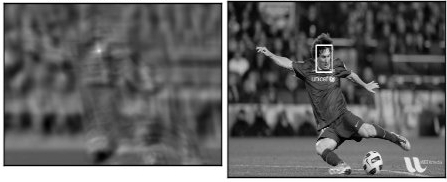
\includegraphics[width=35em]{Images/template_ccoeff_1.jpg}
    \caption{Template matching provides a high level example of a feature (in this case, the template is a face image) and its resulting feature map. (Image taken from \cite{opencv})}
    \label{fig:template_matching}
\end{figure}

\section{Viola-Jones Object Detection Framework}
\label{s:viola}
Now that we have gone over what features and feature maps are, we can begin discussing one of the major sources of inspiration for this thesis, the Viola-Jones Object Detection Framework. This framework is a well known method of image classification and object detection. It has been published in the papers 'Rapid object detection using a boosted cascade of simple features' \cite{viola} and 'Robust Real-Time Face Detection' \cite{viola_updated}, with each having been cited thousands of times, indicating their popularity. When the method was first proposed in 2001, it introduced a system that was extremely efficient and fast, while also maintaining accuracy and robustness. This level of performance was brought about by the introduction of new algorithms and data structures that complimented each other and allowed for great performance gains.

This framework was originally designed to detect faces by sliding a small detection window ($24 \times 24$ pixel resolution) across a larger image, classifying areas as containing a face or not as it went. These classifications were made using Haar-like features, inspired by Haar basis functions. 

\subsection{Haar-like Features}
Haar-like features work by grouping certain areas of pixels into positive and negative regions, then measuring the total differences of pixel intensity between them. For grey scale images (which the Viola-Jones Framework uses), this is simple, but for colour images, there are two different approaches that can be used: the colour could be converted to a single intensity value, thereby changing the image representation to a grey scale one, or the features could be applied to each channel separately.

In terms of structure, Haar-like features take the form of rectangles of varying shapes and sizes, positioned at different points around an input image space or detection rectangle. These main rectangles contain multiple sub-rectangles, with each of them marked as belonging to either a positive or negative region. The values of these features are computed by subtracting the sum of the pixel values covered by the negative regions from the sum of the values in the positive regions. This produces a single value representing the response of the feature at its position in the image. As stated before, these regions are defined by sub-rectangles within the main rectangle feature. In theory, any arrangement (so long as the sub-regions fit together to form one contiguous rectangle) is possible, though in the papers \cite{viola}\cite{viola_updated}, they limited the arrangements to those found in Figure \ref{fig:haar_features}. The allowed arrangements are based off three different filter templates: two-rectangle features (consisting of two equally sized positive and negative regions), three-rectangle features (consisting of three equally sized regions, with the center being positive and its neighbours being negative), and four-rectangle features (where the positive and negative regions are arranged as diagonal pairs). Within the $24 \times 24$ detection window, the constructed features can take any position or aspect ratio, so long as they fit within its bounds and all the internal regions are of equal size.

\begin{figure}
    \centering
    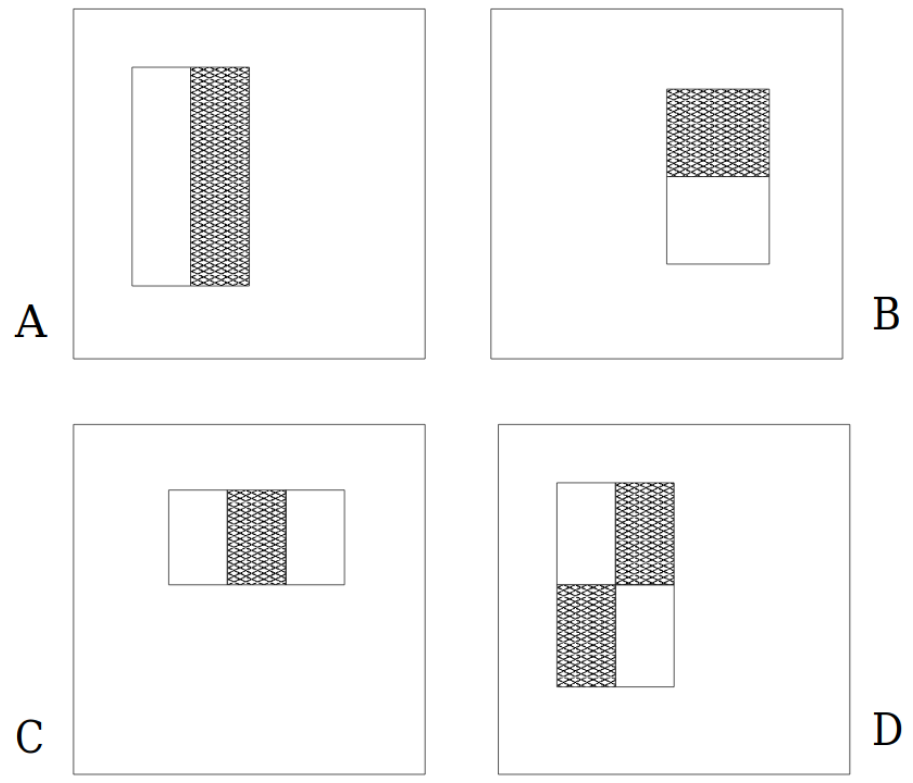
\includegraphics[width=15em, height=15em]{Images/haar_features.png}
    \caption{Examples of Haar-like features. This figure was taken from \cite{viola_updated}. The white regions in these rectangles represent the negative regions, and the black areas represent positive ones. (A) and (B) contain two-rectangle features, (C) contains a three-rectangle feature, and (D) contains a four-rectangle feature.}
    \label{fig:haar_features}
\end{figure}

These features, though the knowledge of them is necessary to understand the Viola-Jones Framework, are not the main contribution of the papers referenced \cite{viola}\cite{viola_updated}. The main innovations here are: A new data structure for the image data (called an integral image), a method for constructing a strong classifier using a handful of features and a variant of the AdaBoost algorithm \cite{adaboost}, and a method of combining increasingly complex classifiers to increase the speed of a detector by focusing on promising regions of the image. 

\subsection{Integral Images}
\label{ss:iimage}
An integral image is a data structure that is extremely well optimized towards the specific task of summing array values within a rectangular area. Since all regions in a Haar-like feature are rectangular in shape, this means that with it, their values can be computed very quickly.

An integral image is created such that the value at every $(x,y)$ coordinate in it is equal to the sum of all the original image intensities above, to the left of, and on the coordinates of the given point. This is formally defined by the following equation.

\begin{equation}
    ii(x,y) = \sum_{x' \leq x, y'\leq y}i(x', y')
    \label{eq:iimage_computation}
\end{equation}

In Equation \ref{eq:iimage_computation}, $ii$ represents the integral image, $i$ represents the original image, and $(x', y')$ and $(x, y)$ represent the original and integral image coordinates, respectively. The main benefit of this approach is that, since each point in the integral image represents a summation of other points, the value of the sum of all points in any arbitrarily positioned rectangle can be computed from the values of only four points on the integral image. An example of this is shown in Figure \ref{fig:integral_computations}. This is formalized using the following equation, where $v$ is the total value of the original image's points within a given rectangle, $x_1$ and $y_1$ are the `top-left' coordinates for said rectangle (Point 1 in Figure \ref{fig:integral_computations}), and $x_2$ and $y_2$ represent the `bottom-right' coordinates (Point 4).

\begin{equation}
    v(x_1, y_1, x_2, y_2) = ii(x_2, y_2) - ii(x_1, y_2) - ii(x_2, y_1) + ii(x_1, y_1)
    \label{eq:iimage_rect}
\end{equation}

\begin{figure}
    \centering
    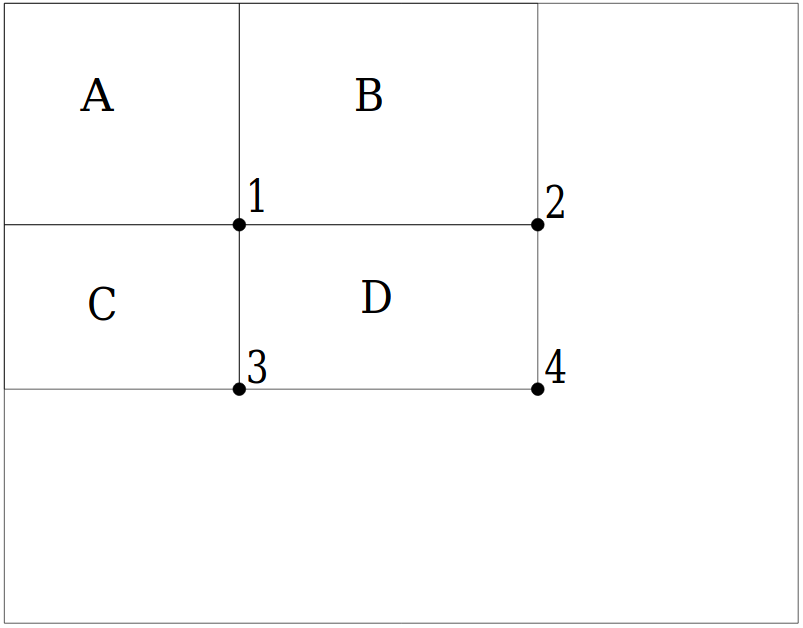
\includegraphics[width=15em, height=15em]{Images/integral_image.png}
    \caption{An example of how the integral image can be computed using only four points (taken from \cite{viola}). Point 1 contains the sum of all values in the region $A$, Point 2 contains the sum of $A$ and $B$, Point 3 contains $A$ and $C$, and Point 4 contains the sum of all values in the labeled regions. Therefore, in order to isolate the value of region $D$, we simply take the value at Point 4, subtract the integral image values of Points 2 and 3, and then add Point 1 to it (the region $A$ would have been subtracted twice since both Points 2 and 3 contain it).}
    \label{fig:integral_computations}
\end{figure}

With this optimization in hand, the features shown in Figure \ref{fig:haar_features} can be computed extremely efficiently, doubly so when the spatial position of the rectangles is leveraged. Since the rectangles are all adjacent to each other, points can be shared, meaning that if the types of Haar-like features being used are known ahead of time, the number of array access operations needed can be reduced. For example, since the rectangles from the two-rectangle example share two of the same points, these only need to be accessed once, reducing the access operation count to 6 instead of 8. 

\subsection{Modified AdaBoost}
The second contribution is the use of an AdaBoost \cite{adaboost} variant for the creation of a strong classifier. The use of this particular approach was made necessary by the extremely large number of possible features that can be constructed using the previously specified Haar-like features. The four rectangular templates, when arranged across the $24 \times 24$ detection window in all possible aspect ratios or positions, produce a total of over 160,000 features \cite{viola_updated} that could be used for classification. This large number means it would be too costly to compute the values of every feature, so an alternative was needed. To this end, a variant of the AdaBoost algorithm was used. The theory behind it is discussed in the following paragraphs.

If we have a set of labeled training data, $\big\{(x_i, y_i)\big\}_{i=1}^{n}$, with an arbitrary distribution, where $x_i$ is a piece of data belonging to (in AdaBoost's simplest configuration) one of two classes $(C_1, C_2)$, and $y_i$ is its label, we wish to make a classifier to classify the data correctly, defined as

\begin{equation}
    h(x) = 
    \begin{cases} 
        1 & \textrm{if  } x \in C_1\\ 
        0 & \textrm{if  } x \in C_2
    \end{cases} .
\end{equation}

This is a difficult problem, and many different methods have been created to attempt to solve it. AdaBoost is one of these approaches, and its basic premise is the idea that many weak classifiers can be combined to form a much stronger classifier. The paper AdaBoost was published in \cite{adaboost} gives the example of a gambler betting on horse races to demonstrate the concept. In this, the gambler is frustrated by continuous losses, and decides to enlist the help of other expert gamblers to increase his winnings. While they are incapable of providing a single master rule for how to bet (classifying horses as winners or losers), they are capable of providing many approximate `rules of thumb' (weak classifiers) that, while very prone to error, still perform better than random chance. By intelligently combining these rules and assigning them weights based on usefulness, the gambler would be able to create his own, much improved, master rule (strong classifier) and be more successful in his betting (make better predictions). This can be formalized as a weighted summation using Equation \ref{eq:strong_classifier_gambler}. 

\begin{equation}
    C(x) = 
    \begin{cases} 
        1 & \textrm{if  } \sum\limits_{t=1}^T \alpha_t h_t(x) \geq \frac{1}{2} \sum\limits_{t=1}^T \alpha_t \\ 
        0 & \textrm{otherwise}
    \end{cases}
    \label{eq:strong_classifier_gambler}
\end{equation}

In this, the strong classifier will only return a positive classification if a weighted majority of the weak classifiers also classify it as positive. Here, $\alpha_t$ represents the weight assigned to an individual, weak classifier, $h_t(x)$. The question then follows, how are these individual classifiers defined and weighted? The original AdaBoost paper \cite{adaboost} gives several methods for this, depending on the configuration, but for simplicity's sake, we will only cover the modified method used in the Viola-Jones paper \cite{viola}\cite{viola_updated}. 

As mentioned before, the different combinations of rectangular feature templates, positions, sizes and aspect ratios produce a sizable number of features. Each of these features can be used to create a single weak classifier that, like a single `rule of thumb' from the gambling example, performs very poorly, but remains slightly better than chance. The way of defining this is formalized in Equation \ref{eq:classifier}.

\begin{equation}
    h_j(x) = 
    \begin{cases} 
        1 & \textrm{if  } p_j f_j(x) < p_i\theta_j \\ 
        0 & \textrm{otherwise}
    \end{cases}
    \label{eq:classifier}
\end{equation}

In this equation, $h_j(x)$ represents the weak classifier, $p_j$ represents the polarity of the feature, and $f_j(x)$ represents the response of the feature itself. $\theta$ is the set threshold that the feature response must surpass in order for the weak classifier to label its input positively.

%This threshold is calculated by creating a list of the training input images and sorting them by the value of the feature's response. The optimal threshold can then be computed in a single pass over the sorted list.

The weights, $\alpha$, for each weak classifier are set to be inversely proportional to the overall error rate when using the selected feature for classification. When classifying, the error $e$ is set to 0 if the classification is correct, and 1 otherwise. This allows the weight for a given classifier to be computed using the following formulae.

\begin{equation}
    \alpha_t = \textrm{log}\frac{1}{\beta_t} \textrm{,\phantom{x}}
    \beta_t = \frac{\epsilon_t}{1-\epsilon_t}
\end{equation}

Where $\epsilon$ represents the total error of the given classifier, summed over each piece of training data. This is formalized as

\begin{equation}
    \epsilon_t = \sum\limits_{i} |h(x_i, f, p, \theta) - y_i| .
\end{equation}

With these formulae, it is possible to create a composite classifier from every feature, weighting them such that the most useful ones contribute more to the final classification than others. Unfortunately, a problem still remains. As mentioned at the start of this section, there are over 160,000 different features that can be used for classification. This is far too many to be able to train in a timely manner or process for real-time computations without exceptionally powerful hardware. Fortunately, there is another optimization that can be made. 

The 160,000 features are composed of rectangles in every position, aspect ratio, and size, but the vast majority of these will contribute very little to the final classifier. It is unlikely, for example, that the two-rectangle feature covering the top-left pixel, and the pixel immediately below it in the detection window will produce any useful predictions at all. As such, if the complex classifier is restricted to using only the top $T$ best performing weak classifiers (200 in the original paper \cite{viola}), the classification performance will remain high, while dramatically reducing the amount of computations needed. The question now becomes 'how do we choose the best performing classifiers?'. 

Obviously, the first step is to iterate over a selection process, picking out the best feature every time, but there is a complication here: the best performing classifiers may all correctly label the same sub-set of the training data, but make similar mistakes that would repeatedly misclassify the remainder. To solve this, the classifiers being selected need to be weighted such that previously misclassified data is given more importance when evaluating the performance of a classifier for selection. As the selection algorithm is iterated through, points that are repeatedly misclassified will be assigned increasingly large weights, ensuring that \textit{eventually} a classifier will be chosen that handles them correctly. This is done by first initializing weights for every piece of data, with the values of either $\frac{1}{2m}$, where $m$ is the total number of negative examples in the training set, or with $\frac{1}{2l}$, where $l$ is the total number of positive examples in the training set. These assignments are based on if the data's label, $y_i$, is negative or positive, respectively.

Once the weights are initialized, the iteration from 1 to $T$ (the desired number of weak classifiers) can begin. At the start, the weights must be normalized using Equation \ref{eq:weight_normalizaiton_adaboost}.

\begin{equation}
    w_{t,i} \leftarrow \frac{w_{t,i}}{\sum^n_{j=1} w_{t,j}}
    \label{eq:weight_normalizaiton_adaboost}
\end{equation}

The selection equation occurs next, though it has to be updated to allow for the weighting of the feature responses.

\begin{equation}
    \epsilon_t = \textrm{min}_{f,p,\theta} \sum\limits_{i} w_i |  h(x_i, f, p, \theta) - y_i|
\end{equation}

Once the selected classifier has been added to the chosen list, the weights are then updated using the equation
\begin{equation}
    w_{t+1, i} = w_{t,i}\beta_t^{1-e_i},
\end{equation}
and the process begins anew. Combining these steps with the previously defined functions yields the final, modified AdaBoost algorithm, as shown in Algorithm \ref{alg:vj_adaboost_algorithm}.

\begin{algorithm}
    \caption{Part 1}
    \label{alg:vj_adaboost_algorithm}
    \begin{algorithmic}
        \addtocounter{algorithm}{-1}
        \Require Example images $(x_1, y_1) ... (x_n, y_n)$ where $y_i = 0$ for negative and $1$ for positive examples.\\
        \item First, Initialize the weights $w_{1,i}=\frac{1}{2m},\frac{1}{2l}$ for $y_i = 0, 1$ respectively, where $m$ and $l$ are the number of negatives and positives respectively.\\
        \For{$t = 1,...,T$}
            \begin{enumerate}
                \item \textrm{Normalize the weights.}
                \begin{equation}
                    w_{t,i} \leftarrow \frac{w_{t,i}}{\sum^n_{j=1} w_{t,j}}
                \end{equation}
                
                \item \textrm{Select the best weak classifier with respect to the weighted error.} 
                \begin{equation}
                    \epsilon_t = \textrm{min}_{f,p,\theta} \sum\limits_{i} w_i |  h(x_i, f, p, \theta) - y_i|
                \end{equation}
                
                \item Define $h_t(x) = h(x, f_t, p_t, \theta_t)$ where $f_t$, $p_t$, and $\theta_t$ minimize $\epsilon_t$. 
                
                \item Update the weights
                \begin{equation}
                    w_{t+1, i} = w_{t,i}\beta_t^{1-e_i},
                \end{equation}
                where $e_i = 0$ if example $x_i$ is classified correctly, $e_i = 1$ otherwise, and $\beta_t = \frac{\epsilon_t}{1-\epsilon_t}$.
            \end{enumerate}
        \EndFor\\\\
        
        The final strong classifier is:
        \begin{equation}
            C(x) = 
            \begin{cases} 
                1 & \textrm{if  } \sum\limits_{t=1}^T \alpha_t H_t(x) \geq \frac{1}{2} \sum\limits_{t=1}^T \alpha_t \\ 
                0 & \textrm{otherwise}
            \end{cases}
            ,
        \end{equation}
        where $\alpha_t = \textrm{log}\frac{1}{\beta_t}$.

        \caption{The boosting algorithm (modified from AdaBoost) used to assemble the strong classifier. It has been taken from \cite{viola_updated}.}
    \end{algorithmic}
\end{algorithm}

\subsection{Attentional Cascade}
The modified AdaBoost algorithm and combination classifier greatly improve efficiency when compared to working with every possible classifier due the assumption that the majority of the features won't be useful. There are still performance gains to be found, however. Strong classifiers assembled using the previous method perform well, but with upwards of 200 weak classifiers needing to be evaluated, they can still be computationally costly. This is especially true when the detection window needs to be slid across a large image. The final major contribution of the Viola-Jones framework, is the concept of an 'Attentional Cascade'. This, again, makes an assumption that unlocks a more efficient approach: The majority of detection windows will be classified as 'negative'. Continuing with the face detection use case, when searching for faces in a large image there may be a handful of them present, but compared to the number of detection window positions covering background or non-face objects, these will be few and far between. Finding a way to discard the windows likely to be negative without evaluating all 200 classifiers could lead to significant decreases in execution time.

This is where the 'Attentional Cascade' idea comes into play. In this, simple classifiers composed of only a handful of features can be used to discard the majority of the irrelevant detection windows. In order for this idea to work, the detection process is organized using a degenerate decision tree (called a `cascade') composed of the low complexity classifiers, with each level of the tree containing a single classifier. At runtime, an input image window is passed through the tree, proceeding to the next level only if the current classifier marks it as positive. If the classifier at any level of the tree marks the window as 'negative', the process immediately stops, the window is discarded, and subsequent classifiers are not activated. This allows the full processing power of the system to only be devoted to areas where there is a high likelihood of a face being present, discarding the others with a minimal number of operations. Since only a tiny fraction of the detection windows in a given image will be positive, with the rest being negative, this leads to a significant improvement in performance.


%These classifiers are created using the same boosting process as before, albeit with many fewer features, and are configured to have very low false-negative detection rates. 

%The final major contribution that this paper makes, is the concept of an 'Attentional Cascade'. Strong classifiers assembled using the previous method perform well, but with upwards of 200 weak classifiers needing to be computed, they can still be costly, especially when the detection window needs to be slid across a large image. That is where the cascade idea comes in. 

%In this idea, simple classifiers can be used to discard many negative instances of the detection window, while allowing almost all the positive instances to remain. 

During the construction of the aforementioned decision tree, the classifiers are trained using AdaBoost, though the given thresholds are chosen such that they minimize false negative detections rather than minimizing the overall error. This necessitates that a low threshold for the classifier is chosen, as higher thresholds decrease the overall error but increase the number of false negatives which, since a false negative early on will cause the window to be discarded, is something that is extremely undesirable. It is also noted that, in order to benefit from the early discarding, the early classifiers must be very simple. In the paper, the first classifier used consisted of only two two-rectangle features (which required roughly 60 microprocessor instructions to compute) but, with the correct threshold set, achieved a 100\% detection rate for faces, with a false-positive rate of 50\% \cite{viola_updated}. While the false-positive rate is high, the paper stated that later classifiers could catch them and noted that scanning templates or single layer preceptrons would be much more computationally expensive (requiring at least twenty times as many operations per window). 

The subsequent classifiers are trained on image windows that have successfully passed through the previous ones, meaning that each classifier gets trained on progressively `harder' windows. Additionally, their complexity also increases. For example, in the paper \cite{viola_updated}, the final detector the authors constructed has its second and third classifiers use 25 features each, and the three following classifiers use 50 features. Though the false positive rate remains high throughout this, and actually increases as the images pass through more and more classifiers, the large number of them (a total of 38 were used), combined with training to correctly classify what the previous classifiers had missed, means that with a deep enough decision tree, the system as a whole can prune these false positives and produce very accurate results. 

\subsection{Viola-Jones Conclusion}
The Viola-Jones Algorithm is accurate and extremely efficient, but it is not without its flaws. The rectangular Haar-like features, while powerful in large numbers, still lack the expressive ability that features from, for example, a modern convolutional net maintain. The feature values are also potentially inconsistent depending on the environment the input image was taken in. Because of their reliance on pixel intensities for computing feature values, Haar-like features are susceptible to lighting variations. Additionally, the system does not handle rotations well, due to the features being rectangular and fixed in either a vertical or horizontal orientation. There are methods that attempt to compensate for these problems, for example, an extension that allows for rotated Haar-like features to handle rotated faces \cite{Rotated_Haar}, but the base system still struggles with these issues. These problems, among others, mean that while the Viola-Jones framework was an excellent algorithm for its time, its accuracy has long since been surpassed by modern methods. Evidence of this is shown in Table \ref{tab:vj_acc}.

\begin{table}[]
\centering
    \begin{tabular}{|c||c|c||c|c||c|} 
        \hline
        \textbf{Detector} & \multicolumn{2}{c||}{\textbf{FDDB data}} & \multicolumn{2}{c||}{\textbf{Casablanca data}} \\ 
         & AUC & mAP(\%) & AUC & mAP(\%) \\
        \hline\hline
        VJ \cite{viola} \textbackslash \space VJ-CRF \cite{VJ_CRF} & 0.6654 & 67.16 & 0.42 & 37.68 \\ 
        \hline
        HeadHunter \cite{HeadHunter} \textbackslash \space DPM \cite{DPM} & 0.7780 & 77.78 & 0.58 & 51.57 \\
        \hline
        \hline
        SSD \cite{SDD} & 0.7740 & 85.00 & 0.68 & 57.57 \\
        \hline
        Faster R-CNN \cite{FRCNN} & 0.9253 & 91.73 & 0.55 & 56.37 \\
        \hline
        R-FCN 50 \cite{RFCN} & \textbf{0.9339} & \textbf{92.92} & 0.63 & 60.53 \\
        \hline
        R-FCN 101 \cite{RFCN} & 0.9287 & 92.53 & 0.63 & 60.67 \\
        \hline
        PVANET \cite{RFCN} & 0.9168 & 91.87 & 0.55 & 60.11 \\
        \hline
        Local-RCNN \cite{LRCNN} & N/A & N/A & \textbf{0.78} & \textbf{71.76} \\ 
        \hline  
    \end{tabular}
\caption{Average AUC (area under curve) and mAP (mean average precision) scores for face and head detection when using the FDDB \cite{ds:FDDB_Dataset} and Casablanca \cite{ds:Casablanca_Dataset} datasets, respectively. Table taken from \cite{Face_detection_Comparison}.}
\label{tab:vj_acc}
\end{table}

As you can see, compared to modern approaches using neural nets, the accuracy of the Viola-Jones framework (denoted by `VJ') is much lower. This is especially true when working on the Casablanca dataset, which measures performance detecting heads in multiple different orientations, not just faces. Were the accuracy metrics used here the only metrics of importance, the method would likely have fallen out of use, but for certain applications, it still persists. Looking at Table \ref{tab:vj_mem} tells us the reason for its persistence. 

\begin{table}[b]
\centering
    \begin{tabular}{|c||c|c|c|c|c|} 
        \hline
        \textbf{Detector} & \multicolumn{2}{c|}{\textbf{Time}} & \multicolumn{2}{c|}{\textbf{Memory}} \\ 
         & \textbf{GFLOPS} & \textbf{FPS} & \multicolumn{2}{c|}{\textbf{consumption (GB)}} \\
        \hline\hline
        VJ \cite{viola} \textbackslash \space VJ-CRF \cite{VJ_CRF} & \textbf{0.6} & \textbf{60.0} & \multicolumn{2}{c|}{\textbf{0.1}} \\ 
        \hline
        HeadHunter \cite{HeadHunter} \textbackslash \space DPM \cite{DPM} & 5.0 & 1 & \multicolumn{2}{c|}{2.0} \\
        \hline
        \hline
        SSD \cite{SDD} & 45.8 & 13.3 & \multicolumn{2}{c|}{0.7} \\
        \hline
        Faster R-CNN \cite{FRCNN} & 223.9 & 5.8 & \multicolumn{2}{c|}{2.1} \\
        \hline
        R-FCN 50 \cite{RFCN} & 132.1 & 6.0 & \multicolumn{2}{c|}{2.4} \\
        \hline
        R-FCN 101 \cite{RFCN} & 186.6 & 4.7 & \multicolumn{2}{c|}{3.1} \\
        \hline
        PVANET \cite{RFCN} & 40.1 & 9.0 & \multicolumn{2}{c|}{2.6} \\
        \hline
        Local-RCNN \cite{LRCNN} & 1206.8 & 0.5 & \multicolumn{2}{c|}{2.1} \\ 
        \hline  
        Yolo 9000 \cite{YOLO9000} & 34.90 & 19.2 & \multicolumn{2}{c|}{2.1} \\ 
        \hline  
    \end{tabular}
\caption{Runtime and Memory consumption when doing face detection using the FDDB \cite{ds:FDDB_Dataset} dataset. Table taken from \cite{Face_detection_Comparison}.}
\label{tab:vj_mem}
\end{table}

Though the framework takes a significant amount of time and memory to train, once it has converged to a solution, its speed and memory efficiency are very good. Even the fastest neural networks in this table are at least thrice as slow, and the most compact, requiring seven times more memory. This means that, when system resources are limited or real-time execution is required, there is still a use for the Viola-Jones framework.

\section{Neural Networks}
As mentioned in the previous section, neural networks are capable of very high accuracy when processing images, with modern architectures surpassing the performance of the Viola-Jones framework by a significant margin. They require large amounts of data to train, but are, in general, much more powerful than classical methods of machine learning for image processing. Unfortunately, this comes at the cost of execution time and memory efficiency. In this section, we will go over their theory and structure, beginning with a definition taken from "An Introduction to Neural Networks" by Kevin Gurney.

"A neural network is an interconnected assembly of simple processing elements, units or nodes, whose functionality is loosely based on the animal neuron. The processing ability of the network is stored in the interunit connection strengths, or weights, obtained by a process of adaptation to, or learning from, a set of training patterns." \cite{nn_book}

As per this definition, a neural network is composed of a collection of neurons (the simplest processing elements) connected together. Unlike its inspiration (a biological neuron), however, they are typically organized in a much more structured way. The most common types of artificial neural nets organize the neurons into a sequence of layers. In these, an input is passed to the first layer of the network, the responses of the first layer's neurons are sent to the second layer, and so on, until the final layer outputs the network's results. There are some architectures that make connections that loop back, or contain other exotic configurations to encourage certain behaviors, but these are beyond the scope of this thesis. As such, we will limit ourselves to only discussing the characteristics of neural networks with regard to simple feed-forward networks. These networks are trained by sending inputs through them, computing the error present in its output, and modifying the network's internal parameters to minimize this error. This is done by estimating a gradient of the error with respect to the network's weights, and then using an algorithm called the `Back-propagation of Error' to update the network's parameters. Once the network has been modified, the process is repeated until a defined end-point is reached. In the following subsections, we will discuss the components of the network and their training methods in detail, starting with their most basic part: the neuron.

\subsection{Neurons}
In its typical form, a neuron maps values from an array of inputs to a single output value. These inputs (and output) usually take the form of floating point numbers, with non-numeric data often being expressed by using embeddings to transform it into one of these forms. These inputs are represented by $x_{0...N}$ in Figure \ref{fig:neuron}, the output is represented by $y$, and $w_{0...N}$ represent the weights in this figure. These weighs are used to modify the inputs before they reach the neuron by multiplying the inputs by themselves. They are often initialized randomly before training begins. Once these inputs have been weighted, they are summed together and passed to an activation function $f(x)$, which determines the neuron's output value $y$. In the earliest uses of a neuron, such as the perceptron, this activation function was a simple threshold, where if the summed input values were greater than a given level, the neuron would output a 1, but if the value was below it, a 0 would be returned instead. This is only the most basic activation function, however, and more complex functions, which we will discuss in the next subsection, are used in modern networks. Additionally, a bias value, $b$, can be used by the neuron to effectively shift the activation function left or right on the graphs shown in Figure \ref{fig:activations}. This is applied just like a weight would be, but for this particular input, the value being multiplied is always equal to 1.  

\begin{figure}[h]
    \centering
    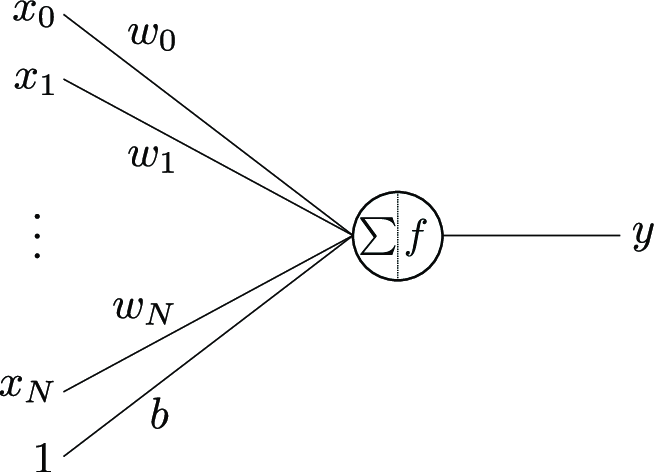
\includegraphics[width=20em]{Images/neuron.png}
    \caption{An diagram of a typical neuron (taken from \cite{neuron_image}, slightly modified). }
    \label{fig:neuron}
\end{figure}

\subsection{Activation Functions}
As mentioned before, one of the components in a neuron is its activation function. This activation function receives the summed values of the neuron's weighted inputs and bias as its input, and can take the form of any unary function. In practice, however, only a few effective ones are commonly used. We will go over the four functions displayed in Figure \ref{fig:activations}, as well as one other, simple function that did not need visualization.

\begin{figure}[h]
    \centering
    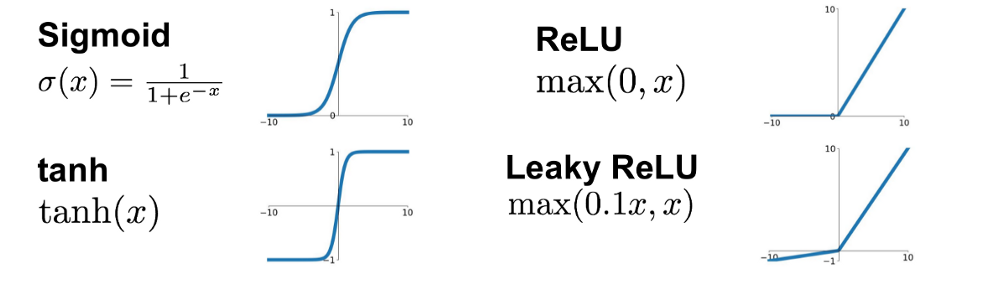
\includegraphics[width=40em]{Images/Activation_Functions.png}
    \caption{Four common activation functions, visualized (taken from \cite{activation_functions}).}
    \label{fig:activations}
\end{figure}

The first function we'll go over is the simplest: the linear activation function. This function is a direct mapping from the sum of the total inputs to the output, formalized as
\begin{equation}
    f(x) = ax.
\end{equation}
Sometimes this is scaled by multiplying the inputs by the value $a$, but it is also possible to leave $a$ equal to 1, so no scaling occurs. This function is very simple to implement, and it works for outputs where the values need to be unrestricted in any direction, but there is a major problem that prohibits its widespread use. The derivative of a linear function is a constant, with no relation in value to the input. This prevents back-propagation from working, since it requires the relationship between an input and the derivative of a neuron's activation function to determine which parameters to improve. 

The second function, shown in the top-right of Figure \ref{fig:activations} is the ReLU, or `Rectified Linear Unit' activation function. As of 2017, this was the most widely used activation function for deep neural networks \cite{searching_for_activation_functions}. It is formalized as
\begin{equation}
    f(x) = 
    \begin{cases} 
        0 & \textrm{if  } x < 0 \\ 
        x & \textrm{otherwise}
    \end{cases}
    .
\end{equation}
While it may look like a linear function, ReLU has a derivative that, though undefined at $x = 0$, allows for back-propagation to work. Its derivative is the step function
\begin{equation}
    f'(x) = 
    \begin{cases} 
        0 & \textrm{if  } x < 0 \\ 
        1 & \textrm{otherwise}
    \end{cases}
    .
\end{equation}
ReLU is very popular mostly because of this, and the fact that it is very efficient to compute. Compared to the Sigmoid and tanh activation functions, there are no expensive exponential or hyperbolic tangent functions to compute, meaning that the networks can be processed faster. The function is not perfect, though. One problem that can occur is that, since the derivative of the function when $x$ is less than 0 is 0, some neurons may not be updated by back-propagation, or activated when the network is used. This can be partially beneficial, allowing for sparser networks that perform faster, but too many dead neurons can harm a network's ability to learn. This problem is addressed with the Leaky ReLU. 

The Leaky ReLU, an extension of ReLU, is the third function we'll go over. It is defined by
\begin{equation}
    f(x) = 
    \begin{cases} 
        ax & \textrm{if  } x < 0 \\ 
        x & \textrm{otherwise}
    \end{cases}
    .
\end{equation}
Here, $a$ is a small value like $0.01$, which solves the problem of neurons never activating, since the derivative when $x < 0$ would be equal to $a$. This does not mean is a guaranteed improvement, however, since it has been shown to not always outperform ReLU \cite{searching_for_activation_functions}. It fixes a problem ReLU has, but does not ensure better performance in all cases.

The last two common functions are the sigmoid and tanh activation functions. The sigmoid function is popularly used when a neural net is designed to classify inputs. It is defined as
\begin{equation}
    f(x) = \frac{1}{1 + e^{-x}},
\end{equation}
for binary classification problems, though it can be modified into a softmax function
\begin{equation}
    f(x) = \frac{e^{x_c}}{\sum_b e^{-x_b}},
\end{equation}
for multi-class problems. Its input, like others, can span the entire input space, but the classifier is most `sensitive' when its inputs are close to 0. Too high or too low of input values are problematic as they would require significant changes in value to cause even minor differences in the activation function's output. This causes the gradient to vanish and makes it extremely difficult for the system to learn. Additionally, due to its use of exponential functions, this activation function is comparatively costly to compute. Despite these flaws, however, the function is still popular for its utility when a network needs to make classifications. Since the outputs are normalized between 0 and 1, this function can conveniently be used to output probabilities for classifications. The function is also smooth, with smooth derivatives, which prevents large jumps in values during training. 

The sigmoid function always outputs a positive number, but sometimes this property is not ideal. The tanh function, defined as
\begin{equation}
    f(x) = \tanh{x}, 
\end{equation}
remedies this by behaving similarly to a sigmoid, except its output values span the space from -1 to 1. That property aside, it has all the same benefits and problems. Its smooth and easy to differentiate, avoiding sudden, large changes in value, but is still computationally expensive and encounters the vanishing gradient problem. 

\subsection{Back-propagation}
\label{ss:backprop}
In the previous sections, we mentioned how neural networks were trained by updating their internal values using the Back-propagation algorithm, and how certain activation functions did not work with it. This algorithm is a fundamental piece of artificial neural networks, so because of its importance, we will go over it here. The algorithm was originally published in a paper titled `Learning representations by back-propagating errors' in 1986 \cite{backprop}, and is described as a procedure that "repeatedly adjusts the weights of the connections in the network so as to minimize a measure of the difference between the actual output vector of the net and the desired output vector." \cite{backprop} 

The difference measurement mentioned here is the network's loss function, which varies depending on its purpose. These can be vast and varied, but common ones are the L1 or L2 loss functions, or as defined by the paper \cite{backprop},
\begin{equation}
    E = \frac{1}{2}\sum\limits_c\sum\limits_j(y_{j,c} - d_{j, c})^2 .
    \label{eq:bp_3}
\end{equation}
Here, $E$ is the error or loss value, $j$ is an index over the unit (neuron) outputs, $c$ is an index over the input-output data pairs, and $d$ is the desired output (the data's labeled ground truth).

With this and the previous definition in hand, we can now go into the details of the back-propagation algorithm. The goal is to update the weights such that, for every input, an appropriate output will be returned that is the same as, or close enough to, the labeled ground truth. For this, an error surface from $E$, is defined with respect to the network's weights, such that the gradient of said surface can be used to determine the way we should modify the weight values. By adjusting these weights, we can descend this gradient, reducing the error and increasing the system's performance. Using this idea of gradient descent, the formula for updating a given weight is defined as
\begin{equation}
    \Delta w = -\epsilon\frac{\delta E}{\delta w} ,
    \label{eq:bp_8}
\end{equation}
where $w$ is a weight and $\Delta w$ is the change to be made to said weight value. $\epsilon$ is a pre-defined value to determine how much the weight should be adjusted with respect to the gradient, otherwise known as a learning rate, and $\frac{\delta E}{\delta w}$ is derivative of the error with respect to the weights, indicating the slope of the gradient of the error surface. Now that we have this formula, the question becomes `How do we get the derivative of it for any weight in the network?'.

Back-propagation is a two-step process. The first step is the forward pass, simply sending a data instance through the network to activate the neurons. The input vectors are weighted and passed to the input neurons, those neurons activate based on their activation functions, and the outputs are passed to the middle layers of the network, otherwise known as the `hidden layers'. The process repeats from layer to layer, until it reaches the output layer and the network returns its final values. This is where the second step, the backward pass, begins and the weights of the individual neurons are updated. Differentiating the loss function, Equation \ref{eq:bp_3}, isolated for a specific input-output index, produces
\begin{equation}
    \frac{\delta E}{\delta y_j} = y_j - d_j .
    \label{eq:bp_4}
\end{equation}
This is the derivative of the error with respect each output neuron, but we need to take a step back and calculate the derivative with respect to an output neuron's total input as well. To get that value, $\frac{\delta E}{\delta x_j}$, the chain rule can be applied to \ref{eq:bp_4}, producing
\begin{equation}
    \frac{\delta E}{\delta x_j} = \frac{\delta E}{\delta y_j} \cdot \frac{\delta y_j}{\delta x_j} .
    \label{eq:bp_4_2}
\end{equation}
This is the derivative of the error with respect to the output neuron's input. In order to solve this, we need to know what $\frac{\delta y_j}{\delta x_j}$ is, but remember, for a neuron, the function $f(x)$ (which produces $y$) is that neuron's activation function. Therefore, we can compute this by taking the derivative of the activation function. In this paper \cite{backprop}, the activation function they used was the sigmoid function, $y = \frac{1}{1 + e^{x}}$. The derivative of this is $y' = y(1-y)$, so the updated representation for $\frac{\delta E}{\delta x_j}$ is
\begin{equation}
    \frac{\delta E}{\delta x_j} = \frac{\delta E}{\delta y_j} \cdot y_j(1-y_j) .
    \label{eq:bp_5}
\end{equation}
This function indicates how the error will change with respect to the inputs for a neuron in the output layer, and from here, we can again apply chain rule to derive a function of how each individual input weight will affect the error. For the weight connecting the neuron $i$ to the output neuron $j$, its effect on the overall error is represented by
\begin{align}
    \frac{\delta E}{\delta w_{ji}}
    & = \frac{\delta E}{\delta x_j} \cdot \frac{\delta x_j}{\delta w_ji} \\
    & = \frac{\delta E}{\delta x_j} \cdot y_i ,
    \label{eq:bp_6}
\end{align}
and the output of a neuron $i$'s effect on $\frac{\delta E}{\delta y_i}$, caused by the cascading effect of $i$ influencing $j$ is defined as
\begin{equation}
    \frac{\delta E}{\delta y_i} = \frac{\delta E}{\delta x_j} \cdot \frac{\delta x_j}{\delta y_i} = \frac{\delta E}{\delta x_j} \cdot w_{ji} .
    \label{eq:bp_6_2}
\end{equation}

Finally, since a non-output neuron will have its output mapped to multiple other neurons, when all weighted connections from the neuron $i$ are considered, the final equation for $\frac{\delta E}{\delta y_i}$ is defined as

\begin{equation}
    \frac{\delta E}{\delta y_i} = \sum_j \frac{\delta E}{\delta x_j} \cdot w_{ji} .
    \label{eq:bp_7}
\end{equation}

This allows us to compute $\frac{\delta E}{\delta y}$ for any neuron in a non-output layer, when the $\frac{\delta E}{\delta y}$s for each neuron in the later layer are provided. By repeating these derivations, we can iteratively compute the derivatives for earlier and earlier layers, allowing us compute $\frac{\delta E}{\delta w}$ as part of the process for each individual weight. With this, we have everything we need to solve Equation \ref{eq:bp_8}.

$\Delta w = -\epsilon\frac{\delta E}{\delta w}$ is a simple and effective method of updating the weights, but it is very slow and takes a long time to converge on an optimal weight configuration. The paper \cite{backprop} therefore proposes an upgrade to this that improves convergence times. This uses an acceleration method, where a weight at a given point on the error surface is modified according to a velocity instead of just its position. The gradients then modify this velocity, using the following formula:

\begin{equation}
    \Delta w(t) = -\epsilon\frac{\delta E}{\delta w(t)} + \alpha \Delta w(t-1)
    \label{eq:bp_9}
\end{equation}

Here, $t$ is increased by 1 for every iteration of the algorithm, and $\alpha$ is an exponential decay factor between 0 and 1 that governs how strongly earlier gradient values affect the current velocity. These modifications means that, if a plateau on the error surface is hit, but previously, the surface had been very steep, the weights will still be modified a significant amount, based on previous values, and won't stall or only update by tiny amounts. Additionally, if the error surface was very steep in the previous time step, and is still steep, the modification to the weights at the current timestep will be even larger than before, allowing it to converge more rapidly. These modifications lead to significantly faster optimization of the network's weights. 

With this formula, now that we have covered how to compute the needed values, our explanation of the back-propagation algorithm is complete.

\subsection{Neural Network Layers}
As mentioned before, a neural network is most commonly organized into a series of layers, with the top layer being the input layer, the intermediate layers being called the 'hidden' layers, and the final layer being the output layer. The internal organization of these layers can take different forms, however, to encourage different behaviors or improve overall performance. In this section, we will go over three important layer structures: the fully connected layer, the convolutional layer, and the pooling layer.

\subsubsection{Fully Connected Layer}

\begin{figure}
    \centering
    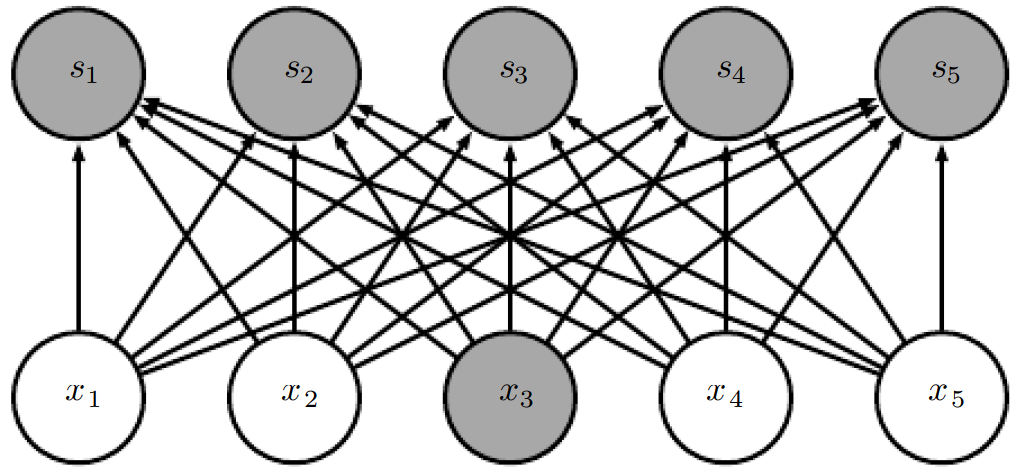
\includegraphics[width=30em]{Images/FC_layer.PNG}
    \caption{An example of a fully connected layer (taken from \cite{dl_book}). Note that the outputs from every $x$ neuron are connected as inputs to every $s$ neuron.}
    \label{fig:fc_layer}
\end{figure}

The fully connected (FC) layer is the most basic type of layer. As demonstrated in Figure \ref{fig:fc_layer}, the output of each neuron in a given layer is taken as an input by every neuron in the subsequent layer. This has the potential to be very powerful, but is extremely computationally expensive, making it inefficient when used as a brute-force solution. Since every neuron is connected to every subsequent neuron, features based on any combination of the inputs can be learned, but this has several problems. 

The first is that, like our filter examples from the Viola-Jones section, the majority of these combinations are going to be useless for the purpose of learning features to classify from. Additionally, even if a useful feature was learned, because of the nature of the FC layer connections, it would not be invariant to translation. Secondly, the number of connections rapidly balloons to absurd levels. Again, referencing the $24 \time 24$ detection windows that the Viola-Jones framework uses, if we were to use two fully connected layers of equal size, where each pixel was represented by a neuron, that would result in $(24 \times 24) \times (24 \times 24)$ connections, producing a total of 331,776 weights that would need to be updated at each step of the learning process. This number of computations would slow the learning and detection rate to a crawl, even more so when we consider that neural networks are rarely only two layers deep. 

Despite these problems, fully connected layers are still commonly used, though not as the main components of a neural net. Often, after the input has been processed by sparser layers, FC layers are used to learn useful combinations of a more limited number of features given by the prior layer's output, and use these to produce a classification. An example of this is the VGG16 network architecture \cite{vgg16}. In this, the majority of the layers are convolutional or pooling layers, with only the final three being fully connected ones. One might look at the number of neurons defined in these, and correctly observe that the $4096 \times 4096$ connections between the first two FC layers would produce 16,777,216 weights, a number far greater than our Viola-Jones example, but its important to note that this network is designed to work with inputs of size $224 \times 224 \times 3$ ($224 \times 224$ RGB images). If the first two layers in it were equally sized fully connected ones, that would produce $(224 \times 224 \times 3) \times (224 \times 224 \times 3)$, or over 22 billion, weights. In comparison to that, approximately 17 million is a significant reduction.

\subsubsection{Convolutional Layer}
The convolutional layer is an answer to the problem of the fully-connected layers being extremely computationally expensive. As indicated by their name, convolutional networks function by using the mathematical operation of `convolution' in place of typical matrix multiplication. They are often used when dealing with data arranged in a grid-like structure, such as image data.

The convolution operation is defined by an asterisk, ie: $I * K$. In this function, the first argument is the input data $I$, which is usually a multidimensional array, and the second is the kernel $K$ (often called a `filter'), a much smaller array that will be applied to the input. The output of this operation, $S$, is a modified version of the input data, sometimes called a feature map. Though this operator does have a generalized definition for infinite functions, in this paper we will restrict ourselves to discussing the definition used when applying the convolution operator to 2d images, as that is one of its most common use cases in the field of deep learning. Said definition for discrete convolution is given as follows:

\begin{equation}
    S(i, j) = (I * K)(i,j) = \sum \limits_m \sum \limits_n I(m, n) K(i - m, j - n) .
    \label{eq:conv_1}
\end{equation}

Figure \ref{fig:conv_example} illustrates how this works in practice in an easy to visualize way. In layman's terms, the convolutional operator slides the kernal matrix across the input matrix, multiplying each input element by the kernel element that overlaps it, and then sums the multiplied elements to produce a new value for the output matrix. This operation is commonly used in computer vision applications, where pre-defined kernels are used to highlight certain edges or textures, respectively, in a given image. 

\begin{figure}
    \centering
    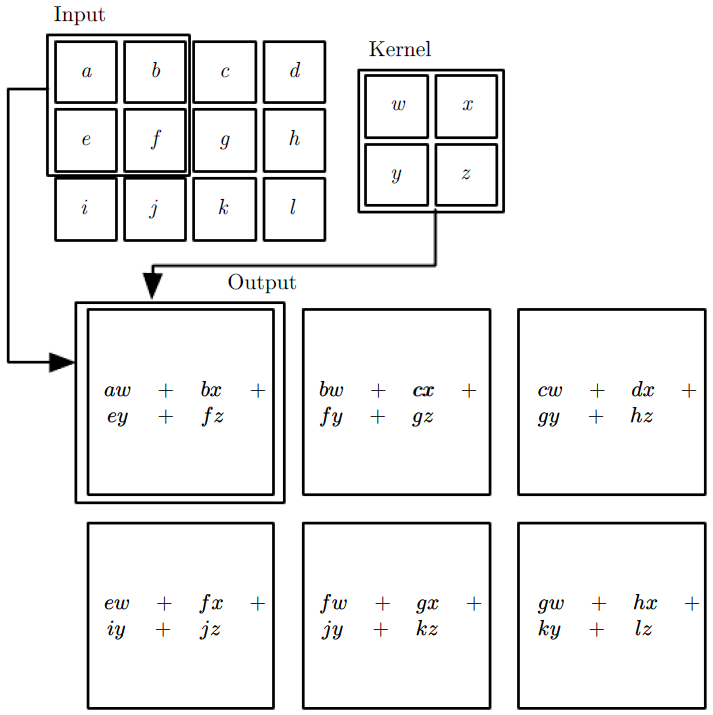
\includegraphics[width=40em]{Images/conv_example.PNG}
    \caption{An example of convolution applied to a 2d grid of data and a smaller $2 \times 2$ kernel (taken from \cite{dl_book}).}
    \label{fig:conv_example}
\end{figure}

A convolutional layer takes this idea and extends it to work with neural networks. In this, it learns sets of kernels (or filters) through its connections and weights. It then uses the convolution operator on these kernels and the input image to produce sets of feature maps indicating the response of each filter. The convolution operation is also often modified by the addition of stride and padding variables. The stride variable changes the amount by which the window shifts in each step of the convolution, and the padding variable pads the input (usually with zeros, duplicated or mirrored input values) around the edges. This padding allows the convolution to be performed on the edges of the input-grid, preventing (or lessening) the shrinking of the final output seen in Figure \ref{fig:conv_example}. This new formulation of a neural network layer promises significant performance increases by encouraging three major ideas: sparse interactions, parameter sharing, and equivariant representations. 

As mentioned before, a fully connected layer has weights connecting every neuron output from one layer to every other input on a second layer. The connections for a convolutional network, however, are much sparser because the kernels they learn are smaller than a given input's size. While an image may be of shape $200 \times 200$, it is not uncommon for individual kernels to only be size $5 \times 5$ as in LeNet-5 \cite{lenet5}, or $3 \times 3$, as in the VGG16 network \cite{vgg16}. 

While it is common whole stacks of kernels to be trained in a modern convolutional layer, in spite of this, there are still many less parameters needed to be updated or stored, and fewer operations are needed to compute an output. For example, the algorithms and matrix multiplications used to process neurons with $m$ inputs and $n$ outputs tend to have a runtime of $O(m \times n)$. These kernels, though, limit the number of connections to $k$, reducing the runtime to $O(k \times n)$. Since $k$ will be significantly smaller than $m$, the overall time complexity will be much smaller and performance will improve significantly \cite{dl_book}. While one may point out that these filters are so small that they would only be able to learn simple features, by stacking many convolutional layers together, the size of the receptive field (the area of the input that a neuron can `see') can be increased. This allows for more complex features to be learned through combinations of the simpler features from the shallower layers.

\begin{figure}
    \centering
    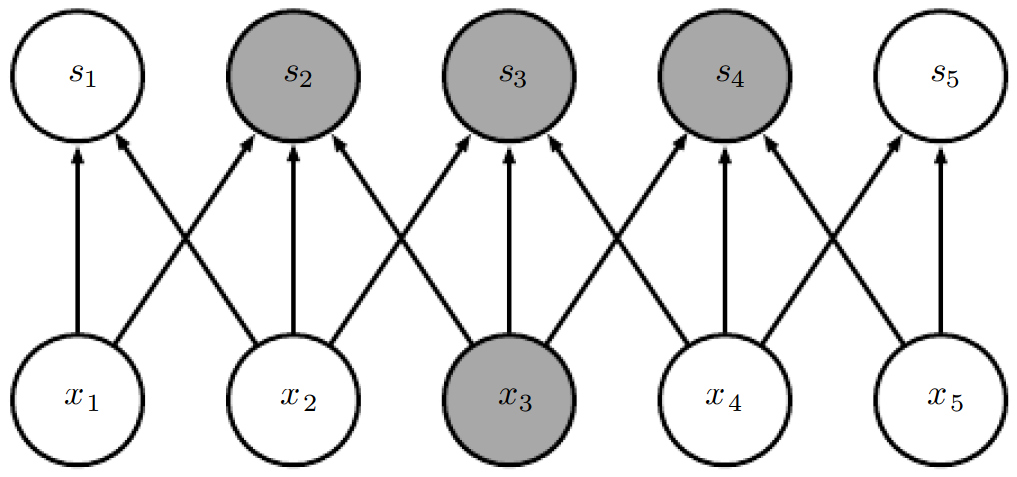
\includegraphics[width=30em]{Images/Conv_layer.PNG}
    \caption{An example of sparse connectivity (taken from \cite{dl_book}). Contrast this to the number of connections found in Figure \ref{fig:fc_layer}, and the reasoning behind the desirability of this property becomes clear - less connections means a faster network.}
    \label{fig:conv_layer}
\end{figure}

The second idea, parameter sharing, is the idea of using the same parameter for multiple operations in a model. In a fully-connected layer, every connection has its own separate weights that need to be stored, leading to a memory complexity of $O(m \times n)$. A convolutional layer does not do this, however. When the kernel is being trained, a set of $k$ weights are learned and then, when the kernel is slid across the layer's inputs for the convolution step, these $k$ weights are reused for their respective connected neurons at each position over and over, until the entire input array has been processed. While this does not affect the time-complexity of the network's operations, since only one set of weights needs to be learned and stored, parameter sharing reduces the memory complexity to $O(k)$. Since $k$ is much smaller than $m \times n$, this greatly increases the memory efficiency of the network.

Lastly, the idea of equivariance is that if the input to a function changes, the output should change in the same way. \cite{dl_book} gives the example of functions $f(x)$ and $g(x)$. In this, $f(x)$ is equivariant to $g(x)$ if $f(g(x)) = g(f(x))$. In the context of neural networks, this means that if an input is modified by anything like, for example, the translation of an input image, then an equivariant network should produce an output that has been likewise translated. A convolutional layer is equivariant for translations because, unlike a fully connected layer, the weights are tied to the sliding window and not directly to the inputs themselves. This means that if a kernel would produce a response to a certain feature in one image, but in a second image, that same feature existed in a translated state, the output from the convolutional layer would be the same, albeit with the response having been returned at the new location.

The convolution operation is, sadly, not equipped to handle changes in rotation or scale without additional extensions, but merely being equivariant to translation is still extremely useful for one of its most common uses: working with image data. In large image datasets or real world applications, it would be unlikely that the same image features would occur in the same places all the time. While a fully connected layer may struggle here, a convolutional layer would be able to pick out similar features across the image with ease, resulting in much greater success. Therefore, by using a layer architecture that is equivariant to translation, the robustness of the network is increased.

\subsubsection{Pooling Layer}

\begin{figure}
    \centering
    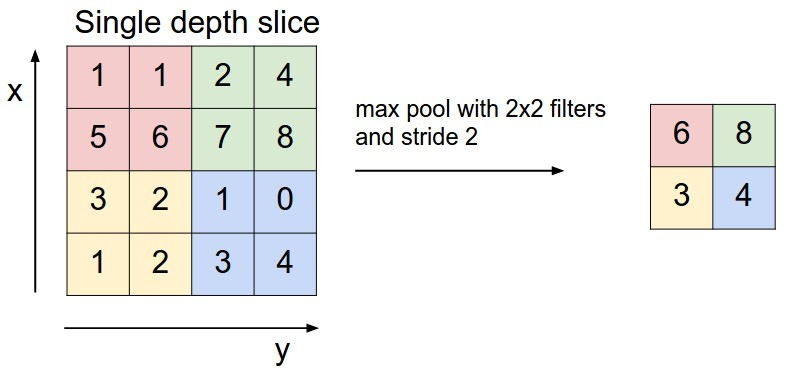
\includegraphics[width=30em]{Images/maxpool.jpeg}
    \caption{An example of pooling using a maximum value function (taken from \cite{max_pool_graphic}). Note how the new $2\times2$ grid is composed of the greatest values from the respectively coloured quadrants in the $4\times4$ grid.}
    \label{fig:max_pool_graphic}
\end{figure}

Convolutional layers perform very well, but sometimes numerous weak responses clutter the feature maps, making it more difficult to work with the most salient, strong feature responses. To solve this problem, an additional part is often inserted into the network after the convolutional layers, before the output is sent to the deeper layers, to improve network performance. This is based off a type of summary-statistics, called a pooling layer.

The pooling layer is not a traditional neural network layer, per say. Indeed, it does not actually contain neurons, nor does it have weight values to adjust during back propagation. Instead, it is simply a mathematical operation applied to the outputs of the neurons in the convolutional layer. Despite this difference, we still refer to it as a `layer' because that is how it is often represented in network architecture diagrams. This layer is defined with a shape and a stride value, and it behaves similarly to a convolutional kernel, sliding a window across the image. At each window position, a function is computed to condense the values from the pooling window down to a single digit. The most common one is to simply return the maximum value within a certain window, which should correspond to the most salient of features output by the prior convolutional layers. This is not the only function, however, others such as the $L^2$ norm of the window's values, or a weighted average based on distance from the center pixel are also popular \cite{dl_book}. 

The use of this addition has two main benefits. Firstly, since the pooling windows condense many values down to a single one, if the stride and shape variables are chosen intelligently, this can improve network efficiency. As per the example in Figure \ref{fig:max_pool_graphic}, a $4\times4$ grid has been condensed to a $2\times2$ grid, while maintaining the strongest features. This will decrease the number of inputs for the following layer, reducing the total computation time. Secondly, pooling the grid like this strengthens the network's invariance to small translations of the input. When configured for returning the maximum value, so long the desired feature response is present, it does not matter where in a given window it is, the output of the layer will be the same. This increases the network's robustness and learning ability. 

\subsection{Training a Neural Network}
So far we have discussed how networks are constructed, their components, the algorithms used, and some important datasets and architectures, but we haven't gone into detail on the actual training process yet. Training uses the method of gradient descent to optimize the weights and biases of a network, and over the course of many iterations, slowly converges on a state that will maximize the accuracy of its outputs. As mentioned in Section \ref{ss:backprop}, an error surface is computed during the process of back propagation, and by observing the slope of this surface (the gradient), we can adjust the network such that it slowly descends this slope, lowering its error and increasing its overall accuracy. To do this, we use an optimization function like Stochastic Gradient Descent (SGD) or the Adam method. 

Originally, when using back propagation to update the network, the entire training dataset would be provided at once. This meant the gradient with respect to every piece of data would need to be computed for a single update which, when dealing with large datasets, was impractical at best and impossible at worst. SGD was a solution to this, where random, non-repeating points would be drawn from the dataset and the network would be updated based on a single instance. The process would then be repeated with new points until the dataset was exhausted. This did mean that the gradients varied significantly between training iterations, making the optimization more difficult, but the updates were much faster and required far less memory. This was then further refined with the use of batches, where small chunks of the dataset would be used to calculate the gradients instead of individual pieces. This helped to reduce the amount of variation in the gradient between updates, while maintaining reasonable speed and efficiency. Adam is another version of this process, which only calculates first-order gradients during its computation process, allowing for a lower memory requirement, as well as several other benefits to improve the learning process \cite{adam}.

This training process is guided by a series of parameters set when the network is defined, including a learning rate, a momentum value, a weight decay parameter, and an input batch size. As mentioned in Section \ref{ss:backprop}, the learning rate governs how quickly the network descends the gradient. A larger value allows the weights to shift by larger amounts, and a smaller value limits the amount of change a weight can undergo. The momentum value is an attempt to solve the problem of the gradient descent process getting stuck on local minima. In this, the rate of change from the previous step is used as a parameter to determine the amount the weights are going to be updated in the current step. For example, if the gradient is very steep in one iteration, but very shallow in the next, some of the steepness will be maintained as a portion of the current gradient calculations. The weight decay parameter is used as a method of regularizing network models. It prevents network weights from growing too large by being set to a value less than 1, and multiplying itself against the weights after each training step to shrink them. Lastly, the batch size is the number of entities from the training dataset that will be used to train the network in a given step using the previously mentioned gradient descent and optimization algorithms.  

The training process iterates through random, non-repeating batches of the dataset, updating the network in each step, until it manages to process all the data. Only stepping through the dataset a single time, though, often isn't enough to properly train the network, especially if the learning rate is low. As such, the network will return to the start of the dataset, draw new batches containing previously seen data, albeit in random, likely new, combinations, and continue its training. Each loop through the entire dataset is called an `epoch', and dozens to hundreds of them can be required to fully train a network. A pause between epochs is usually where the network's current performance is evaluated, to see how the training is going. The datasets provided to a network are split into training and evaluation subsets, with the training dataset being used to train the network, while the evaluation dataset is unseen during training, and only used to test performance. Between these epochs, the model being trained is locked to prevent updates, then fed batches from the evaluation dataset to see how its solution generalizes to unseen data, before returning to continue its training. Once the network is deemed `fully trained', the evaluation data is run through it one last time to get its final accuracy, and that, along with the evaluation results recorded between epochs, gives the user a good representation of the true performance of the network. Said performance is heavily dependant on the model architecture chosen, however, so picking the best one for the task at hand is critical to the network's success. Since the architecture chosen is so important, in the next section, we will detail several of them.

\subsection{Important Architectures}
\label{ss:important_architectures}
In previous subsections, we went over the components of a neural net and different types of layers. In this, we will discuss how these components can be combined to make modern neural network architectures. Of course, given the field's current popularity, there are a truly immense number of different architectures that have been published, used and iterated upon. Even if we restrict these networks to ones purpose built for image processing related tasks, the number is still staggeringly large. As such, we will restrict ourselves to discussing the three architectures most relevant to this thesis: VGG-16\cite{vgg16}, VGG-7 \cite{ternary}, and LeNet-5\cite{lenet5}.

\subsubsection{LeNet-5}
\label{sss:lenet5}
LeNet-5 is the simplest architecture we'll discuss, consisting of two convolutional layers (each followed by an average pooling layer), and two fully connected layers. A visualization of this is shown in Figure \ref{fig:lenet_architecture}. This architecture is one of the earliest in the history of neural nets, and that, as well as it being very simple, makes it a commonly used architecture to teach the concepts of deep learning using neural networks. It has also found particular success in solving the problem of recognizing hand-written text. In 1989, it was applied to a dataset of handwritten zip codes provided by the U.S. Postal Service to solve the problem of hand-written digit recognition. The resulting performance was a great success, showing its utility in solving real-world problems\cite{lenet_postal_service}.   

\begin{figure}
    \centering
    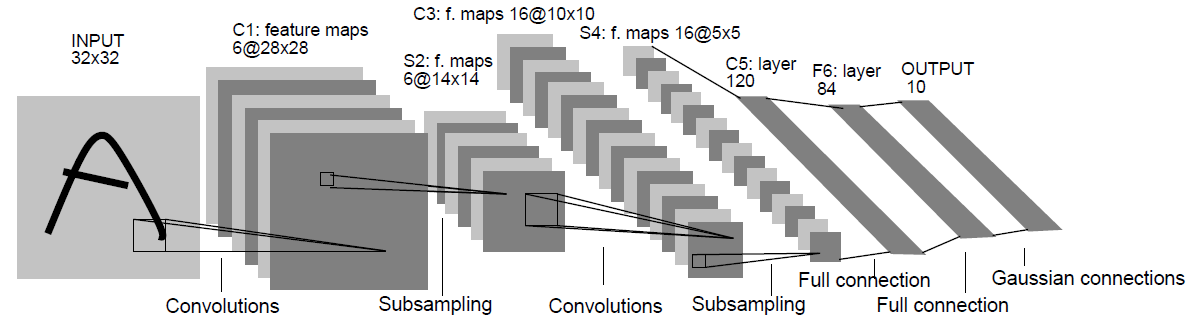
\includegraphics[width=45em]{Images/lenet_architecture.PNG}
    \caption{The LeNet-5 architecture, visualized (taken from \cite{lenet5}). In this diagram, the subsampling sections are the average pooling layers, and the Gaussian connections represent the final soft-max activation function}
    \label{fig:lenet_architecture}
\end{figure}

In its original paper \cite{lenet5}, the first layer of this network is a convolutional layer. This layer takes a $32 \times 32$ sized input and learns six different $5 \times 5$ kernels, then passes the outputs from the kernels to a pooling layer. The pooling layer is defined with a window size of $2 \times 2$, and a stride of 2. This is labeled as `subsampling' in Figure \ref{fig:lenet_architecture}. The function used here for the pooling is defined as one that sums the window values together, multiplies them by a trainable value, and then adds a trainable bias, before applying a sigmoid function to the output. Though the paper \cite{lenet5} uses this psuedo-averaging function for its pooling, other implementations have shown that the architecture works with max-pooling as well \cite{ternary}. The third layer is a second convolutional layer consisting of 16 learnable kernels, again of size $5 \times 5$, and like before, its output is passed into a second pooling layer, identical to the first. Once this has been completed, the features extracted by this set of convolutional and pooling layers are then passed to a pair of two fully connected layers. Here, the relations between the features, and the resulting classifications are learned. 

The first of these is technically another convolutional layer, with 120 kernels of size $1 \times 1$. This size, though, effectively makes it perform like a fully connected layer, so it is sometimes represented as such in network diagrams. The reasoning behind this design decision was that it allowed for the expansion of the network. If the input size were increased, the sizes of the feature maps would increase as well, and this final map's shape would be greater than $1 \times 1$ \cite{lenet5}. The second layer has no special alterations, and performs exactly as one would expect a fully connected layer to. It consists of 84 neurons connected to the 10 units of the output layer, though these output units are not the usual type of neuron. They are defined as Radial Basis Function (RBF) units, where their outputs are formalized as follows:
\begin{equation}
    y_i = \sum\limits_j(x_j - w_{ij})^2 .
\end{equation}
This results in each unit outputting the Euclidean distance between its respective input vector and a parameter vector, with the further the distance, the larger the returned value. Each of these output units represent a class (a number from 0 to 9), and for a given input image, a classification will be returned as the class with the lowest output value. It is worth noting that this method of output is not the only way LeNet-5 has been implemented. While the original paper uses the RBFs for its output units \cite{lenet5}, other methods like softmaxes or support vector machines have been used \cite{ternary}.

\subsubsection{VGG16}
In contrast to the very simple LeNet-5 architecture, VGG16 \cite{vgg16} is a much more complex network with a far greater capacity to learn. Its claim to fame is that it achieved the rank of 1st place in the ImageNet Large Scale Visual Recognition Challenge 2014 (ILSVRC2014) \cite{VGG16_challenge}. The key to this success was its depth (shown in Figure \ref{fig:VGG16_architecture}). Its 13 3-channel convolutional layers and 3 fully connected layers at the end gave it a very high learning capacity and produced exceptional results. The use of such a deep network was made possible by restricting the sizes of the convolutional filters to $3 \times 3$, though because of the number of connections present, it does require a significant amount of memory and computational power to process \cite{binary}.

\begin{figure}
    \centering
    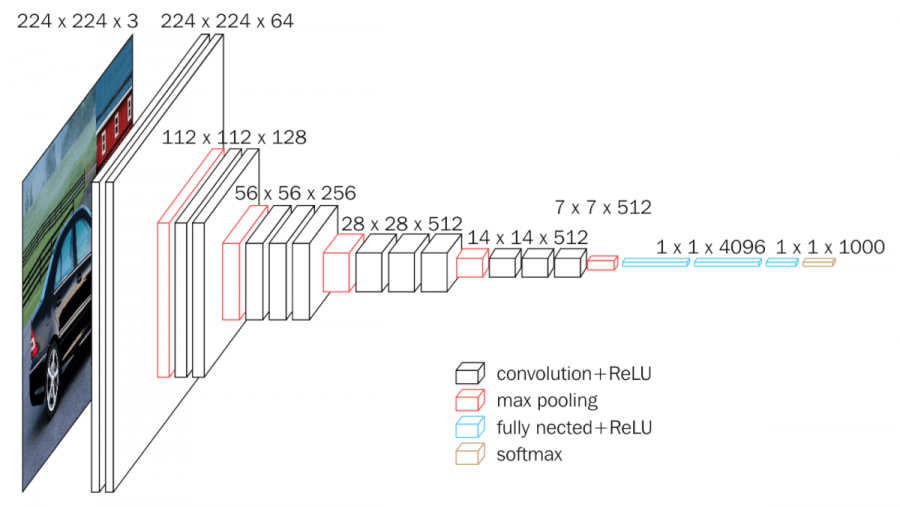
\includegraphics[width=40em]{Images/VGG16.png}
    \caption{The VGG16 architecture (taken from \cite{VGG16_graphic}).}
    \label{fig:VGG16_architecture}
\end{figure}

As shown in \ref{fig:VGG16_architecture}, the convolutional layers are arranged in groups of two for the first two layers, then three for the remainder, followed by a pooling layer using the max value function. The max-pooling layers are defined using a pooling window of size $2 \times 2$, and a stride value of 2. The convolution layers train an increasing number of $3 \times 3$ kernels, beginning at 64 per layer for the first set, then doubling after every pooling layer until they finally reach a set of 512 kernels in the final convolutional layer. From there, a final max-pooling operation happens, and the condensed features are passed to a trio of fully connected layers (consisting of 4096, 4096, and 1000 neurons, respectively). For every layer between the input and output (the `hidden' layers), ReLU activation functions are used, and at the end, a softmax function is used to classify the output.

\subsubsection{VGG7}
\label{sss:VGG7}
The last network we'll discuss is the VGG7 architecture. This is not at all a popular architecture, in fact, it was custom designed for the paper `Ternary Weight Networks' \cite{ternary}, presumably to decrease the memory and computational requirements of the model. It is defined similarly to VGG16, however it is only seven layers deep, with the convolutional layers always being arranged in pairs. The first two layers are the expected pair of $3 \times 3$ convolutional layers, however these each train 128 filters instead of the 64 specified in the original VGG16. The evolution of the remaining convolutional layers proceed as expected, with the number of filters doubling after each max-pooling step, though at the end, they only use a single fully-connected layer before applying a soft-max function for classification. In summary, this network is defined by "$2 \times (\textrm{128-C3}) + \textrm{MP2} + 2 \times (\textrm{256-C3}) + \textrm{MP2} + 2 \times (\textrm{512-C3}) + \textrm{MP2} + \textrm{1024-FC} + \textrm{Softmax}$".  

\subsection{Binary Networks}
\label{ss:binary}
As mentioned before, deep neural networks like VGG16 can be very powerful, but come with the downside of requiring significant computational power and memory resources to run them. As such, they are only suitable for use on expensive, high performance machines. In order to allow these networks to run on weaker machines or mobile devices, alterations needed to be made to the architecture to reduce the hardware requirements. Of the manifold alterations that have been researched, this section will focus on the two most relevant to this thesis: Binary \cite{binary} and Ternary \cite{ternary} networks.

Binary networks are the less relevant of the two, so we will not exhaustively detail them, but their basic concepts are still important for understanding their extension, ternary networks. The main idea is that the weights (and inputs) of a network's neurons can be approximated with binary values. `XNOR-Net: ImageNet Classification Using Binary Convolutional Neural Networks' \cite{binary} proposed two different methods of using these approximations. The first, called a binary weight network, only converted the weight values of the network to binary. In this, they found that switching from single-precision values to simpler, binary values resulted in a network approximately $32\times$ smaller than a standard network, in terms of memory, due to requiring only a single bit for storage. Additionally, they found that since binary weights meant that network operations could be estimated using only addition and subtraction, without computationally expensive multiplication operations, a $2\times$ increase in speed could be achieved while maintaining similar accuracy to a standard network. 

The paper's second method is an extension of this first one, called an `XNOR-Network'. In this, the neuron inputs, as well as the weights, are converted to binary values, which allows for much more efficient computations. If all the operations are done using binary, the network values can be computed using XNOR gates and bitcounting instead of additions and subtractions. This change in operations does result in a less accurate network, but it significantly decreases the required computation time (approximately $58\times$ speed increase for CPU execution). A summary of these statistics is found in Figure \ref{fig:binary_net}.

\begin{figure}
    \centering
    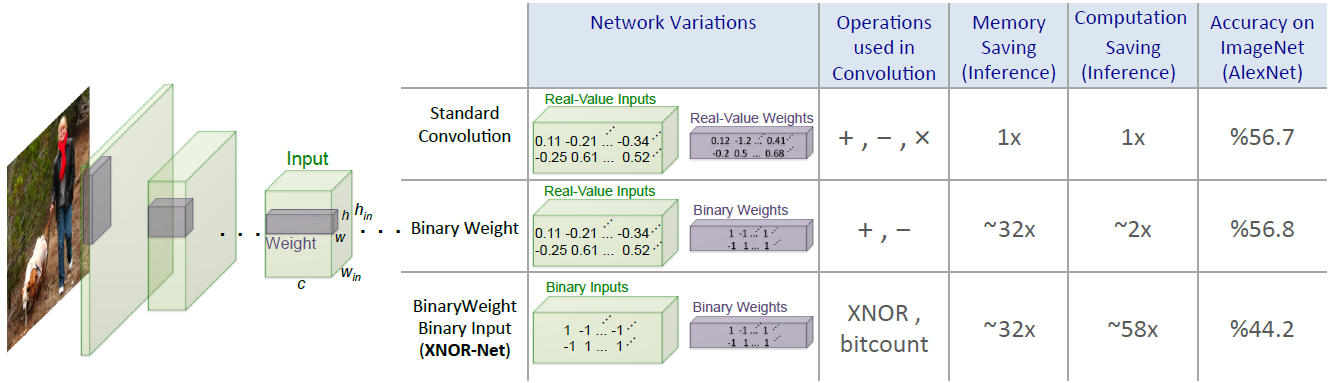
\includegraphics[width=40em]{Images/Binary_Net_Chart.PNG}
    \caption{A comparison of the two different approaches to binary networks, and a standard convolutional network baseline, detailed in \cite{binary} (figure taken from \cite{binary}).}
    \label{fig:binary_net}
\end{figure}

\subsection{Ternary Networks}
\label{ss:ternary}
As said before, ternary networks are an extension of binary weight networks. While binary weight networks produce large gains in memory and computational efficiency, they do come at the cost of learning capacity. Ternary networks, which use three values ($-1$, 0, and 1) instead of the two ($-1$ and 1) that binary networks use, are proposed as a compromise between them.

For $3 \times 3$ convolutional filters, a binary network is capable of representing 512 different filters ($2^{3 \times 3}$), however, a ternary network, with its extra value, is capable of expressing 19683 ($3^{3 \times 3}$) different filters. This, approximately $38\times$, increase in expressive ability allows for the network to learn more complex patterns and improves its performance on complex datasets. Unfortunately, the increase in power comes at the cost of model compression. Since ternary networks use an extra value, they need two bits for storing a single weight instead of one. Therefore, while the binary network can achieve a $~32\times$ reduction in memory use compared to standard models, a ternary network can only achieve a $~16\times$ reduction. This is still a significant increase in memory efficiency however, which the paper \cite{ternary} asserts is good enough. Fortunately, the speed-up given by a binary weight network is not affected by the addition of the extra value. Since the third added value is a 0, the values these are assigned to as weights can simply be ignored, thus allowing the network to operate using only additions or subtractions. This allows a ternary weight network to operate with the same level of computational efficiency as a binary weight network, though the paper \cite{ternary} does not compare this to the much quicker XNOR-Net extension \cite{binary}.

\subsubsection{Ternary Weight Minimization Problem}
\label{sss:ternary_minimization}

When constructing a ternary network, the goal is to minimize the difference between the ternary and the full precision weights that would be trained for the network. In the paper \cite{ternary}, this difference is represented by the Euclidean distance and the minimization problem is defined in Equation \ref{eq:ternary_problem}.

\begin{equation}
    \begin{cases} 
        \alpha^* , W^{t*} = &  \argmin \limits_{\alpha, W^t} J(\alpha, W^t) = ||W - \alpha W^t ||_{2}^{2}\\ 
        \textrm{s.t.} & \alpha \geq 0, \; W^t_i \in \{-1, 0, 1\}, \; i = 1,2,...,n
    \end{cases}
    \label{eq:ternary_problem}
\end{equation}

In this equation, $W$ represents the full precision weights, $W^t$ represents the ternary weights, and  $\alpha$ is a non-negative scaling factor. Since it is assumed that the full precision weights will be approximately equal to the ternary weights (when appropriately scaled), the paper \cite{ternary} uses the approximation $W \approx \alpha W^t$ to define a basic forward propagation step in Equation \ref{eq:ternary_forward_block}.

\begin{equation}
    \begin{cases} 
        Z  & = X * W \approx X * (\alpha W^t ) = (\alpha X) \bigoplus W^t \\ 
        X^{\textrm{next}} & = g(Z)
    \end{cases}
    \label{eq:ternary_forward_block}
\end{equation}

In this, $X$ represents the inputs, $*$ represents a convolution or inner product, $g$ represents a nonlinear activation function, and $\bigoplus$ is an inner product or convolution without multiplication. $X^{next}$ is the output of the step, which will be passed to the next step in the forward pass. In order to compute this, though, the minimization problem from Equation \ref{eq:ternary_problem} needs to be solved.

Unfortunately there is no way to perfectly determine the optimal solution for Equation \ref{eq:ternary_problem}. Expanding $J(\alpha, W^t)$ and deriving with respect to $\alpha$ and $W_i^t$ would not produce independent $\alpha^*$s and $W_i^{t*}$s, so the system has no deterministic solution. As such, an approximation is needed, and the paper \cite{ternary} introduces a threshold-based function to allow for this, shown in Equation \ref{eq:ternary_threshold}. In this equation, $\Delta$ represents a positive threshold value.

\begin{equation}
W_i^t = f_t(W_i|\Delta) = 
    \begin{cases} 
        +1, & \textrm{if} \;W_i\phantom{|} \; > \; \Delta \\
        \phantom{-}0, & \textrm{if} \;|W_i| \; \leq \; \Delta\\
        -1, & \textrm{if} \; W_i\phantom{|} \; < \; -\Delta 
    \end{cases}
\label{eq:ternary_threshold}
\end{equation}

Using this equation, the minimization problem from Equation \ref{eq:ternary_problem} can be rewritten as Equation \ref{eq:ternary_rewrite}.

\begin{equation}
\alpha^*,\Delta^* = \argmin\limits_{\alpha \geq 0, \; \Delta > 0} (|I_\Delta|\alpha^2 - 2(\sum\limits_{i \in I_\Delta} |W_i|)\alpha + c_\Delta)
\label{eq:ternary_rewrite}
\end{equation}

In this, $I_\Delta = \{i \big| |W_i| > \Delta\}$, $|I_\Delta|$ is the number of elements in $I_\Delta$, and $c_\Delta = \sum\limits_{i \in I^c_\Delta} W_i^2$ is an $\alpha$-independent constant. All of these combined together means that, when given any $\Delta$, the approximation of the optimal $\alpha$ can be computed using Equation \ref{eq:ternary_alpha}.

\begin{equation}
\alpha^*_\Delta = \frac{1}{|I_\Delta|}\sum\limits_{i \in I_\Delta} |W_i|
\label{eq:ternary_alpha}
\end{equation}

This can then be substituted into Equation \ref{eq:ternary_rewrite} to produce Equation \ref{eq:ternary_delta}.

\begin{equation}
\Delta^* = \argmax\limits_{\Delta > 0} \frac{1}{|I_\Delta|}(\sum\limits_{i \in I_\Delta} |W_i|)^2
\label{eq:ternary_delta}
\end{equation}

Unfortunately, Equation \ref{eq:ternary_delta} is difficult to solve. A solution can be computed using discrete optimization, but the process is very time consuming, making it impractical. Therefore, the paper \cite{ternary} instead makes the assumption that $W_i$ values are drawn from either a uniform or normal distribution. In a uniform distribution, the authors find that $\Delta^* = \frac{2}{3}E(|W|)$, and in a normal distribution, they compute that $\Delta^* = \frac{3}{4}E(|W|)$. Thus, they pick a mid-point for the coefficient in front of $E$, resulting in Equation \ref{eq:ternary_delta_final}.

\begin{equation}
\Delta^* \approx 0.7 \cdot E(|W|) \approx \frac{0.7}{n}\sum\limits_{i=1}^n |W_i|
\label{eq:ternary_delta_final}
\end{equation}

With this collection of equations in hand, the minimization problem from Equation \ref{eq:ternary_problem} can be approximately solved, allowing the network to function. During training, the ternary network will use full-precision weights for the parameter updates, but during the forward and backward passes between them, it will convert the weights to ternary values. Thus, while a ternary network behaves similarly to a full-precision network during training, once completed, it will operate entirely using the ternary weights (as no further updates will happen), allowing the speed-up and efficiency gains to manifest.

\subsubsection{Ternary Weight Network Performance}
In the paper \cite{ternary}, the authors ran several experiments on the MNIST \cite{mnist}, CIFAR-10 \cite{cifar}, and ImageNet \cite{imagenet} datasets to evaluate the performance of ternary weight networks. In these, they used stochastic gradient descent, a variant of gradient descent that updates after each batch (a randomized subset of input images) instead of each epoch (an iteration through the entire dataset), to train the networks. They also used optimization tricks such as batch normalization \cite{batch_norm} (a method of normalizing a network's inputs), learning rate decay (reducing the learning rate by a factor of 10 after a certain number of iterations to allow for the fine-tuning of the network), and momentum (a modification to gradient descent that helps it avoid local minima) to improve network performance. The experiment parameters are shown in Table \ref{tab:ternary_param}.

\begin{table}
\centering
    \begin{tabular}{c c c c} 
        \hline
         & MNIST & CIFAR-10 & ImageNet \\ 
        \hline
        network architecture & LeNet-5 & VGG-7 & ResNet-18(B) \\
        weight decay & 1e-4 & 1e-4 & 1e-4 \\
        mini-batch size of BN & 50 & 100 & 64$(\times 4)^2$ \\
        initial learning rate & 0.01 & 0.1 & 0.1 \\
        learning rate decay epochs & 15, 25 & 80, 120 & 30, 40, 50 \\
        momentum & 0.9 & 0.9 & 0.9 \\
        \hline

    \end{tabular}
\caption{The parameters used for evaluating the ternary weight network on multiple different datasets (taken from \cite{ternary}).}
\label{tab:ternary_param}
\end{table}

For the MNIST \cite{mnist} dataset, the authors maintained a similar structure to the LeNet-5 architecture discussed in Section \ref{sss:lenet5}, however they did make some changes. For one, the convolutional layers have different numbers of filters. The first layer learns 32 different filters, and the second learns 64 (though still with the filters being of size $5\times5$). Additionally, the first fully connected layer uses 512 neurons, and the final hidden layer, as well as the Gaussian connections, have been replaced with a support vector machine (a machine learning algorithm often used for classification). This was trained for approximately 30 epochs.

For the CIFAR-10 \cite{cifar} dataset, we have already discussed the network structure used. The VGG7 architecture mentioned in Section \ref{sss:VGG7} was designed by the authors explicitly for this experiment. One thing that does need to be mentioned are the modifications done to the inputs. The input images were padded on all sides with four pixels, and this data was augmented by making $32\times32$ random crops and horizontal flips to artificially increase the amount of `new' data the network would see and improve the features that it would learn. This was trained for approximately 170 epochs.

For the ImageNet \cite{imagenet} dataset, the ResNet-18 \cite{resnet} architecture was used. We have not mentioned this architecture before, but as it is not relevant to the main topic of this thesis, we need not go into detail. All that must be known is that it is a powerful, 18-layer deep network composed mostly of convolutional layers. The input data for this network was also augmented with random $224\times224$ crops. This was trained for approximately 55 epochs.

\begin{table}
\centering
    \begin{tabular}{c c c c c} 
        \hline
         & MNIST & CIFAR-10 & ImageNet(top-1) & ImageNet(top-5) \\ 
        \hline
        Ternary Weight Networks & \textbf{99.35} & \textbf{92.56} & \textbf{61.8 / 65.3} & \textbf{84.2 / 86.2} \\
        Binary Weight Networks & 99.05 & 90.18 & 57.5 / 61.6 & 81.2 / 83.9 \\
        \cline{2-5}
        Full Precision Networks & 99.41 & 92.88 & 65.4 / 67.6 & 86.76 / 88.0 \\
        \hline
    \end{tabular}
\caption{Validation accuracies as percentages. Table taken from \cite{ternary}.}
\label{tab:ternary_results}
\end{table}

Table \ref{tab:ternary_results} displays the results of these experiments. As seen here, ternary weight networks come much closer to the accuracy of full precision networks than their binary counterparts. Since these networks still allow for increased model compression and computational efficiency, this compromise between binary and full precision networks seems to be effective.

\section{Datasets}
The available image datasets for training neural networks are extremely varied, with hundreds having been constructed for task-specific problems. These can range from vast image sets with thousands of categories for large-scale image classification problems, to smaller sets consisting of only a pair of image types (eg. face or non-face for a facial recognition dataset). Much like the number of different network architectures, documenting all of these would be an exhausting task, so for this section, we will follow a method similar to what we did in Section \ref{ss:important_architectures}. Instead of detailing all of them, we will focus on the two datasets most relevant to this thesis, the CIFAR-10 and MNIST datasets. These are simple, but popular datasets that were used for the author's experiments in the paper defining ternary networks \cite{ternary}, as well as by us for the same purpose in this thesis. 

\subsection{MNIST}
The MNIST dataset \cite{mnist} is composed of 70,000 images of handwritten digits within the range 0 to 9. These are split into two groups, with 60,000 being used for training a network, and 10,000 being used for evaluation. This dataset was designed to be easy to work with, allowing users to rapidly test pattern recognition algorithms and neural networks without having to process or format the data much on their own. The images in this dataset have only a single dimension (greyscale), and are of uniform size ($28 \times 28$). Their values span the range of 0 to 255, with 0 representing the blank image backgrounds, and larger numbers representing the pixels composing the written digits. Examples of images from this dataset are detailed in Figure \ref{fig:mnist_examples}.

\begin{figure}
    \centering
    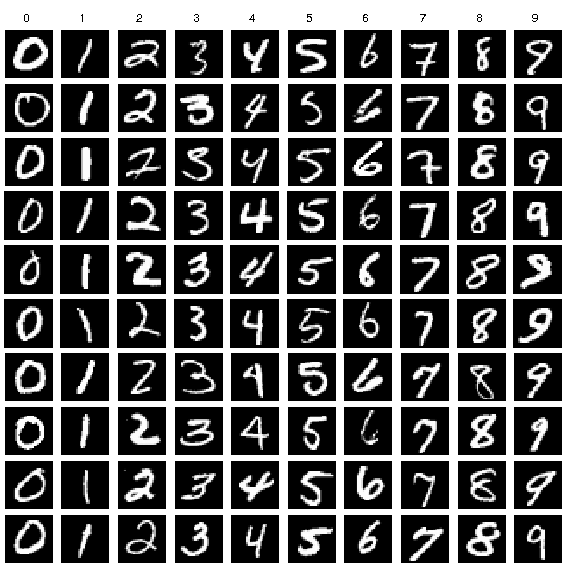
\includegraphics[width=30em]{Images/Example-images-from-the-MNIST-dataset.png}
    \caption{Example images from the MNIST Dataset (figure taken from \cite{ds_analysis}).}
    \label{fig:mnist_examples}
\end{figure}

\subsection{CIFAR-10}
Compared to MNIST, the CIFAR-10 dataset is a more complex set of images that is useful for measuring the performance of networks on harder classification tasks. The dataset contains 60,000 three-dimensional (colour) images evenly spread across 10 different classes (6,000 per class), with a training/test split of 50,000 and 10,000. The images are of size $32 /times 32$, and each belong to one of the following classifications, based on their subjects: airplane, automobile, bird, cat, deer, dog, frog, horse, ship, truck. There is also an extended CIFAR-100 dataset, with 100 classes grouped into 20 superclasses, but neither we, nor the ternary network paper \cite{ternary} used this. Examples of the images from CIFAR-10 are shown in Figure \ref{fig:cifar_examples}.

\begin{figure}
    \centering
    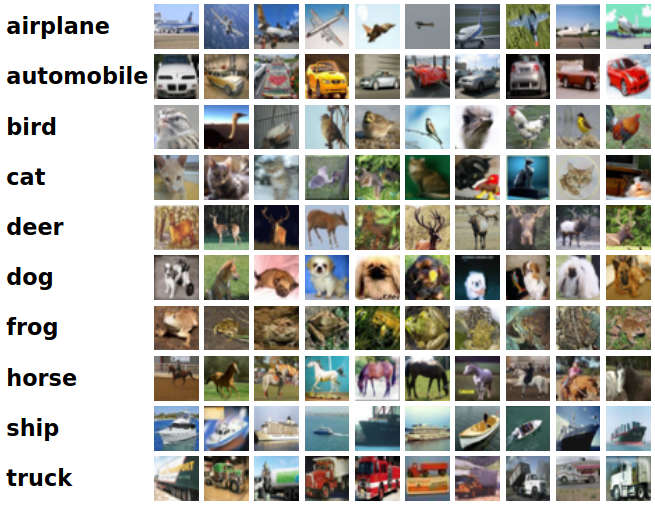
\includegraphics[width=30em]{Images/cifar_examples.png}
    \caption{Example images from the CIFAR-10 Dataset (figure taken from \cite{cifar-image}).}
    \label{fig:cifar_examples}
\end{figure}

\section{Motivation}
As mentioned in Section \ref{ss:ternary}, ternary weight networks are capable of significantly decreasing a network's memory requirements, and slightly increasing its computational efficiency without sacrificing too much accuracy when compared to a full precision network. This is a good start, but we believe that there are additional gains in efficiency that this network architecture can afford. Consider the Haar-like features used in the Viola-Jones framework discussed in Section \ref{s:viola}. These consist of positive and negative regions within a detection window, and the space not covered by these regions is ignored. When compared to the positive, negative, and zero weights attached to the filters of a ternary convolutional layer, the two seem very similar. We believe that by combining the integral image and the structure of the Haar-like features from the Viola-Jones framework with the convolutional layers of a ternary network, even larger speed-ups can be achieved without sacrificing accuracy. In the next chapter, we will go over a process of combining the two, as well as some experimental results detailing the performance and accuracy of the networks.


\chapter{Methodology}
How can one combine the computational efficiency of the Viola-Jones framework with the learning and classification abilities of a convolutional neural network? As mentioned before, the key here lies within the weights of the network and the input data. If we use a ternary network, we can replace the weights of the top-most layer with Haar-like features of similar dimensions and, when applied an integral image, can compute the first layer of the network much more efficiently. The way we accomplish this is detailed in the following section. 

\section{Combination Process}
We start this process by first creating a ternary network according to the architecture we desire. This is functionally the same as creating a full-precision network, except that a conversion from the full-precision to the ternary weights takes place before the forward and backward passes. This conversion is done using the $\alpha$s and $W^{t}$s computed from the equations in Section \ref{sss:ternary_minimization}. Once the ternary network is trained for a given dataset, we then visualize the weights from the first layer. These $n \times n$ weight matrices consist of complex patterns of 0s, 1s, and $-1$s scattered around the grid, as shown by Figure \ref{fig:ternary_example}. Though their values exist within the same ranges as those found in Haar-like features, it is important to note that the Haar-like features consist of up to 4 rectangular subregions, and their rectangular shapes are explicitly required to get any benefit from using an integral image over an ordinary image. As such, the ternary weights need to be modified such that they can be represented by up to four rectangles.   

\begin{figure}
    \centering
    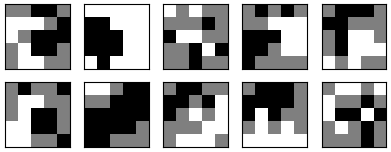
\includegraphics[width=25em]{Methodology_Images/ternary_example.png}
    \caption{A set of example ternary weights (grey represents 0 values, white represents -1, and black represents 1). Note the scattered structure of the weight values. In its current state, this cannot take advantage of the integral image to increase computational efficiency.}
    \label{fig:ternary_example}
\end{figure}

For each filter, we defined a set of new weights by hand. We did this by first searching for large, unbroken patches of singular values that could be covered by one rectangle, or alternatively, for imperfect areas that were still predominantly composed of one value over the others. In each of these spaces, we would define a rectangular patch using the area's top-left and bottom-right $x$ and $y$ coordinates. These patches would then be assigned a value the same as the majority of the weights they covered. While this could (and often does) lead to some weights being assigned values different than what the network learned, so long as the majority (rounding up) of them are correct, it does not seem to harm the network's accuracy significantly. In the case of no large, near-perfect patches being present (like the middle example on the top row of Figure \ref{fig:ternary_example}), we would attempt to maximize expressive ability by selecting four small areas or individual weights based on whatever patterns were currently observed. For every filter, we would try to define four separate rectangular regions, and any weight left uncovered would be set to 0. Only in the cases where less than four rectangles could cover the entity of the positive or negative weights, would we define fewer than this number. Modifying our example weights from Figure \ref{fig:ternary_example} with these rules produces the weights seen in Figure \ref{fig:ternary_block_example}. 

Though the custom weights have been visualized in the same manner as a convolutional filter here, in our actual implementation, we use a list containing only the previously mentioned $x$ and $y$ coordinates of the two corner points from each rectangular region, as well as their assigned value. These coordinates allow for the easy computation of values from the integral image (the details of which were mentioned in Section \ref{ss:iimage}), allowing us to increase our processing speed. If we had only modified the convolutional filters rather than using these coordinate lists, the layer would have behaved exactly the same as a normal convolutional layer (albeit with altered weights), resulting in no speedup. 

\begin{figure}[h]
    \centering
    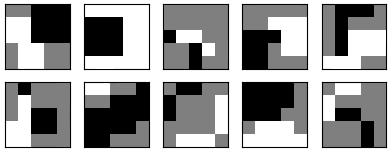
\includegraphics[width=25em]{Methodology_Images/ternary_block_example.png}
    \caption{The ternary weights from Figure \ref{fig:ternary_example}, now grouped into rectangle patches. Admittedly, a certain level of detail has been lost, but the use of these rectangle patches allows for faster computation.}
    \label{fig:ternary_block_example}
\end{figure}

Once these custom filters have been defined, we have to retrain the network to ensure a good level of accuracy. First, though, we remove the top convolutional layer and replace it with a function that behaves just like one, but has been designed to use the previously mentioned coordinate lists as its `filters'. The values in this function are fixed, so they will not be updated during the second training step. Additionally, we also modify the network's input, such that every image sent to the network is transformed into the integral images required by our custom layer function. This allows the value of each `convolutional kernel' to be computed much quicker. We will justify this claim in the next section.


%With these custom weights defined, we then retrained the network, but fixed the weights in the first layer. Those would not be updated during training, instead, during initialization, each weight would be assigned a fixed value based on its position within our manually defined filters. After this second training step, we discard the first layer of the network entirely and replace it with a function that computes the integral image of a given input image. This function then uses the $x$ and $y$ coordinates defined in our custom features to compute the values of their regions, and therefore, the value of each convolutional kernel as a whole, much quicker. We will justify this claim in the next section.

\section{Performance Details}
\subsection{Integral Images}
The definition of an integral image has already been given in Equation \ref{eq:iimage_computation}, but the number of operations that this implies are required is, at first glance, misleading. The naive approach would be to compute the value at every coordinate of the integral image by summing all previous values, but this is inefficient and neglects to take advantage of previous computations by using prior integral values. If we compute each point in an integral image using the following formulae, we can compute non-edge values using 4 array look-ups and 3 mathematical operations, edge values with 2 array look-ups and 1 mathematical operation, and the starting value with a single array look-up. As usual, in these equations, $ii$ represents the integral image, $i$ represents the original image, and $x$ and $y$ represent the coordinates that the value is being computed for. 

\begin{equation}
    ii(x, y) = 
    \begin{cases} 
        ii(x, y) = i(x, y) + ii(x - 1, y) + ii(x, y - 1) - ii(x - 1, y - 1) & \textrm{if } x > 1, \; y > 1 \\
        ii(x, y) = i(x, y) + ii(x, y - 1) & \textrm{if } x = 1, \; y > 1 \\
        ii(x, y) = i(x, y) + ii(x - 1, y) & \textrm{if } x > 1, \; y = 1\\ 
        ii(x, y) = i(x, y) & \textrm{if } x = 1, \; y = 1 
    \end{cases}
    \label{eq:iimage_efficient_comp}
\end{equation}

Observing these equations, we can then calculate the total number of operations that computing an $n \times m$ integral image would require using the following formulae.

\begin{equation}
    \textrm{Ops}_{ii} = \textrm{Array}_{ii} + \textrm{Math}_{ii}
    \label{eq:iimage_num_ops}
\end{equation}

\begin{equation}
    \textrm{Array}_{ii} = 4(n - 1) + 4(m - 1) + (2n - 1) + (2m - 1) - 1
    \label{eq:iimage_num_arr}
\end{equation}

\begin{equation}
    \textrm{Math}_{ii} = (n - 1) + (m - 1) + 3(n - 1)(m - 1)
    \label{eq:iimage_num_math}
\end{equation}

\subsection{Custom Filters}
As shown in Equation \ref{eq:iimage_rect} of Section \ref{ss:iimage}, integral images allow for the computation of any rectangle with a maximum of 4 array look-ups and 3 mathematical operations. Since we have constrained our custom filters to use the same number of rectangles that Haar-like features have ($\leq$ 4), and are working with ternary weights (thus eliminating the need for multiplication) this means that a filter's value can be computed in a maximum of
\begin{equation}
    \textrm{Ops}_\textrm{filter} = 4(4 + 3) = 28
\end{equation}
total operations, regardless of filter size. 

\subsection{Regular Ternary Filters}
Now that we have determined the complexity of our custom filters using haar-like features, we will evaluate the complexity of an ordinary filter from a ternary convolutional layer for comparison. These filters have the same benefit as before, of not requiring the multiplications of the weights on their input vectors, but do not take advantage of the integral image's data structure to improve efficiency. For these $i \times j$ filters, they must compute the feature's value using each input value individually, meaning that $i \times j$ array look-up operations must be used, as well as $(i \times j) - 1$ mathematical operations. This means that, unlike the custom filters, the number of required operations scales with filter size. For example, while a $3 \times 3$ filter is technically more efficient than our custom implementation ($3 \times 3$ look-ups and $3 \times 3 - 1$ operations only results in 17 operations total), as filters get larger, its number of required operations rapidly increases beyond that. The next common size, a $5 \times 5$ filter, requires $5 \times 5$ look-ups and $5 \times 5 - 1$ operations, making a total of 49 operations - a value significantly higher than what our custom filters need.

\subsection{Efficiency Comparison}
\label{ss:efficiency_comp}
Of course, though we can see that our custom filters are individually less expensive to compute than a regular ternary filter of size $5 \times 5$ or greater, there is some additional overhead in the form of the integral image computations. As such, in this section, we will compare the total number of operations needed for a single filter to process a $28 \times 28$ greyscale image.

As mentioned before, our custom filters require a flat 28 operations to compute their values, regardless of their size. Since we are using a convolutional network, these filters will be slid across the image, and therefore, for an image of size $n \times m$, with sufficient padding to avoid shrinking the size of the output, and an stride value of 1, a single filter can compute its feature map in $28nm$ operations. For this scenario, the image would require $28\cdot 28 \cdot 28 = 21952$ total operations to be processed.

For integral images, the number of operations needed to compute them is simple to calculate using the formulae from Equations \ref{eq:iimage_num_ops}, \ref{eq:iimage_num_arr}, and \ref{eq:iimage_num_math}. Using them, a $28 \times 28$ greyscale image would require 325 array look-up operations and 2241 mathematical operations, making a total of 2566. By summing these and the filter operations together, we can get the total number of operations required for computing a feature map, which is 24518.

For the ternary filters, no integral image computation is needed. As such, their total required operations can be defined by simply adding their look-up ($i \times j$)  and mathematical ($(i \times j) - 1$) operations formulae together, followed by multiplying them by the total number of positions the filter will be shifted across ($n \times m$). For $3 \times 3$ filters, this results in 13328 operations, for $5 \times 5$, this requires 38416, and $7 \times 7$ filters need 76048. This means that $3 \times 3$, $5 \times 5$ and $7 \times 7$ custom filters, combined with their integral image, require $1.84\times$, $0.64\times$, and $0.32\times$ as many operations, respectively, when compared against ternary filters. While our solution is slower when computing the less expressive, smaller filters, this shows that for larger ones, it promises significant performance gains. These results are summarized in Table \ref{tab:res_comparison}.

\begin{table}
\centering
    \begin{tabular}{|c c c c|} 
        \hline
         & $3 \times 3$ & $5 \times 5$ & $7 \times 7$ \\ 
        \hline
        Integral Image Operations & 2566 & 2566 & 2566 \\
        Custom Filter Operations & 21952 & 21952 & 21952 \\
        Total Operations & 24518 & 24518 & 24518 \\
        \hline
        Ternary Filter Operations & 13328 & 38416 & 76048 \\
        \hline
        \textbf{(Total Custom / Ternary)} & \textbf{~1.84} & \textbf{~0.64} & \textbf{~0.32} \\
        \hline
    \end{tabular}
\caption{A comparison of number of computations required for a single filter to process a $28 \times 28$ greyscale image, depending on the method used. For each filter size, it is assumed that the padding value is large enough to produce a feature map of the same size as the input. The final row of this table shows the difference in operations between the custom filter and a ternary filter as a ratio.}
\label{tab:res_comparison}
\end{table}


\chapter{Experiments}

While these calculations clearly show improved computational efficiency, this is only useful if the network's accuracy remains at an acceptable level. To determine if our solution meets this requirement, in this section, we will detail a set of experiments we conducted, as well as their results. 

For these experiments, we used two popular datasets to evaluate two different network architectures. The MNIST \cite{mnist} dataset was used to train a variant of the LeNet-5 \cite{lenet5} architecture, and the CIFAR-10 \cite{cifar} dataset was used with the VGG-7 \cite{ternary} architecture mentioned in Section \ref{sss:VGG7}. We chose these datasets and architectures firstly because of their simplicity. MNIST and CIFAR-10 consist of small, uniformly formatted images that are complex and diverse enough to be capable of demonstrating network's learning abilities, but due to their small size, are able to be processed very quickly. Likewise, the LeNet-5 and VGG-7 architectures are quick to compute, but are powerful enough to provide an accurate indication as to the capabilities and limitations of our method. Additionally, we have already seen that they are suitable for the task of evaluating new neural net, since they were used in the ternary networks paper \cite{ternary}.

\subsection{LeNet-5 and MNIST}
Our LeNet-5 network was defined using the same architecture the ternary networks paper \cite{ternary} uses, with one minor difference. For the final layer, where the ternary LeNet-5 uses a support vector machine, we have replaced this with a ten neuron, fully connected layer, where the index of the highest value is the classification that is given to the MNIST number. For parameters, the network uses the Adam algorithm for optimization with a weight decay of 1e-5, and a learning rate of 0.001. For inputs, the network's batch size is set to 100, with the data being normalized to help improve network performance. While some of these settings are different from those specified in the previously mentioned paper \cite{ternary}, it is important to note that the differences do not matter significantly. As all of our LeNet-5 experiments use this same network setup, the comparisons made will still be valid for showing relative performance improvements or shortcomings. 

\subsection{VGG7 and CIFAR-10}
Our VGG7 network is again, defined using the same architecture as the ternary networks paper \cite{ternary}, with a minor modification. As mentioned in Section \ref{sss:VGG7}, its architecture can be summarized as "$2 \times (\textrm{128-C3}) + \textrm{MP2} + 2 \times (\textrm{256-C3}) + \textrm{MP2} + 2 \times (\textrm{512-C3}) + \textrm{MP2} + \textrm{1024-FC} + \textrm{Softmax}$". The key difference here, is that our modification expands the first layer. Instead of it being a $3 \times 3$ convolutional layer, we have increased its size to $5 \times 5$. This is because we already know $3\times3$ layers are more efficient than our custom Haar-like filters, so it makes little sense to evaluate them when the speed/accuracy tradeoff is guaranteed to work in their favour. This network uses Stoicastic Gradient Descent (SGD) as its optimization algorithm, with a learning rate of 0.1, a momentum value of 0.9, and a weight decay parameter of 1e-4. For inputs, it uses a batch size of 100, as well as normalizing and augmenting the batch data with random crops and horizontal flips to encourage it to learn more generalizable features. The last parameter, the learning rate decay, is set to divide the given rate by 10 after 80 and 120 epochs, in order to fine-tune the network and improve overall accuracy.  

\subsection{Network Variations}
For each of these general architectures, five different networks are trained: a full precision network, a full ternary network, an N1T network, a custom full ternary network, and a custom N1T network. The full precision and full ternary networks are, as their names suggest, networks implemented entirely using full precision or ternary weights, respectively. The custom ternary network is a ternary network where we have replaced the weights of the first layer with our custom Haar-like filter functions. The N1T and custom N1T networks are full precision networks, except for the first layer, which has been replaced by a ternary convolutional layer. N1T uses a set of learned ternary weights for this, while the custom N1T network uses our custom filters. The differences between these weights have been visualized in Figure \ref{fig:mnist_combined}.

\subsection{Empirical Run-time}
Though we have already computed the theoretical efficiency gains of our method using several formulae in Section \ref{ss:efficiency_comp}, we also wanted to make some empirical benchmarks to see how long these filters took to process in comparison to standard ternary ones in the real world. For this, we wrote a custom script in Cython to simulate a single-threaded application running both types of convolutional layers. To produce results that are closer to real-world performance, we modeled this implementation after the LeNet-5 model used in the ternary network's paper \cite{ternary}, rather than the original published implementation \cite{lenet5}. This means that the layer we time uses 32 $5 \times 5$ filters instead of the original paper's recommendation of 6. We also included the calculations of the integral image in our timings for the custom filters to ensure our observations are accurate. This experiment was conducted using 500 images from the MNIST dataset. We recorded the individual processing times of each of these images (or, in the case of our custom filters, the conversion time for the integral image \textit{as well as} the network's processing time), then summed them together and divided by 500 to record the average processing time for a single image. This average, computed over a large number of data points, minimizes the influence of outliers in our recordings, and means that the numbers we report are more accurate.

\begin{figure}
    \centering
    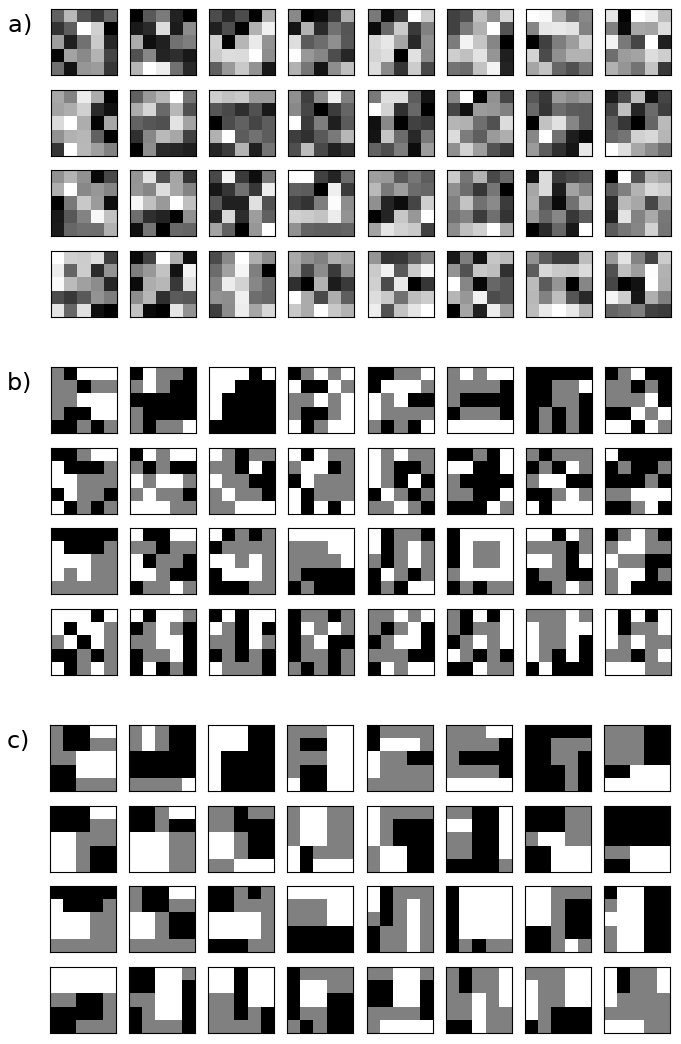
\includegraphics[width=40em]{Methodology_Images/MNIST_Combined_Filters.png}
    \caption{
    The convolutional kernels/filters used for the first layer of LeNet-5 in the MNIST experiment. a) The full-precision filters, b) The trained ternary filters, c) The custom filters, defined by hand}
    \label{fig:mnist_combined}
\end{figure}


\chapter{Results and Discussion}
\section{Results}
The results of our experiments can be seen in Table \ref{tab:res_max_accuracy}, and plots of the accuracies with respect to the number of training epochs can be found in Figure \ref{fig:mnist_accuracy} and Figure \ref{fig:cifar_accuracy}. In our experiments, the ternary networks routinely make less accurate classifications than full precision networks, as expected, but the networks using our custom filters did not deviate significantly from the levels given by standard ternary layers. Even when the networks were very shallow (such as with LeNet-5), where our custom filters would represent a greater proportion of the network, they did not hamper performance. Indeed, in both of the instances where we used our custom layers with the LeNet-5 architecture, as well as the custom N1T instance of VGG7, the networks actually performed slightly better than their ternary counterparts. 

\begin{table}[h]
\centering
    \begin{tabular}{|c|c|c|} 
        \hline
        & LeNet-5 on MNIST & VGG7 on CIFAR-10 \\
        \hline
        Full Precision & 99.36 & 92.41 \\
        Full Ternary & 95.11 & 91.59 \\
        N1T & 99.31 & 91.87 \\
        \hline
        Custom Full Ternary & 95.49 & 91.30 \\
        Custom N1T & 99.48 & 91.90 \\
        \hline
    \end{tabular}
\caption{Validation accuracies (\%) from the different networks and datasets.}
\label{tab:res_max_accuracy}
\end{table}

\begin{figure}
    \centering
    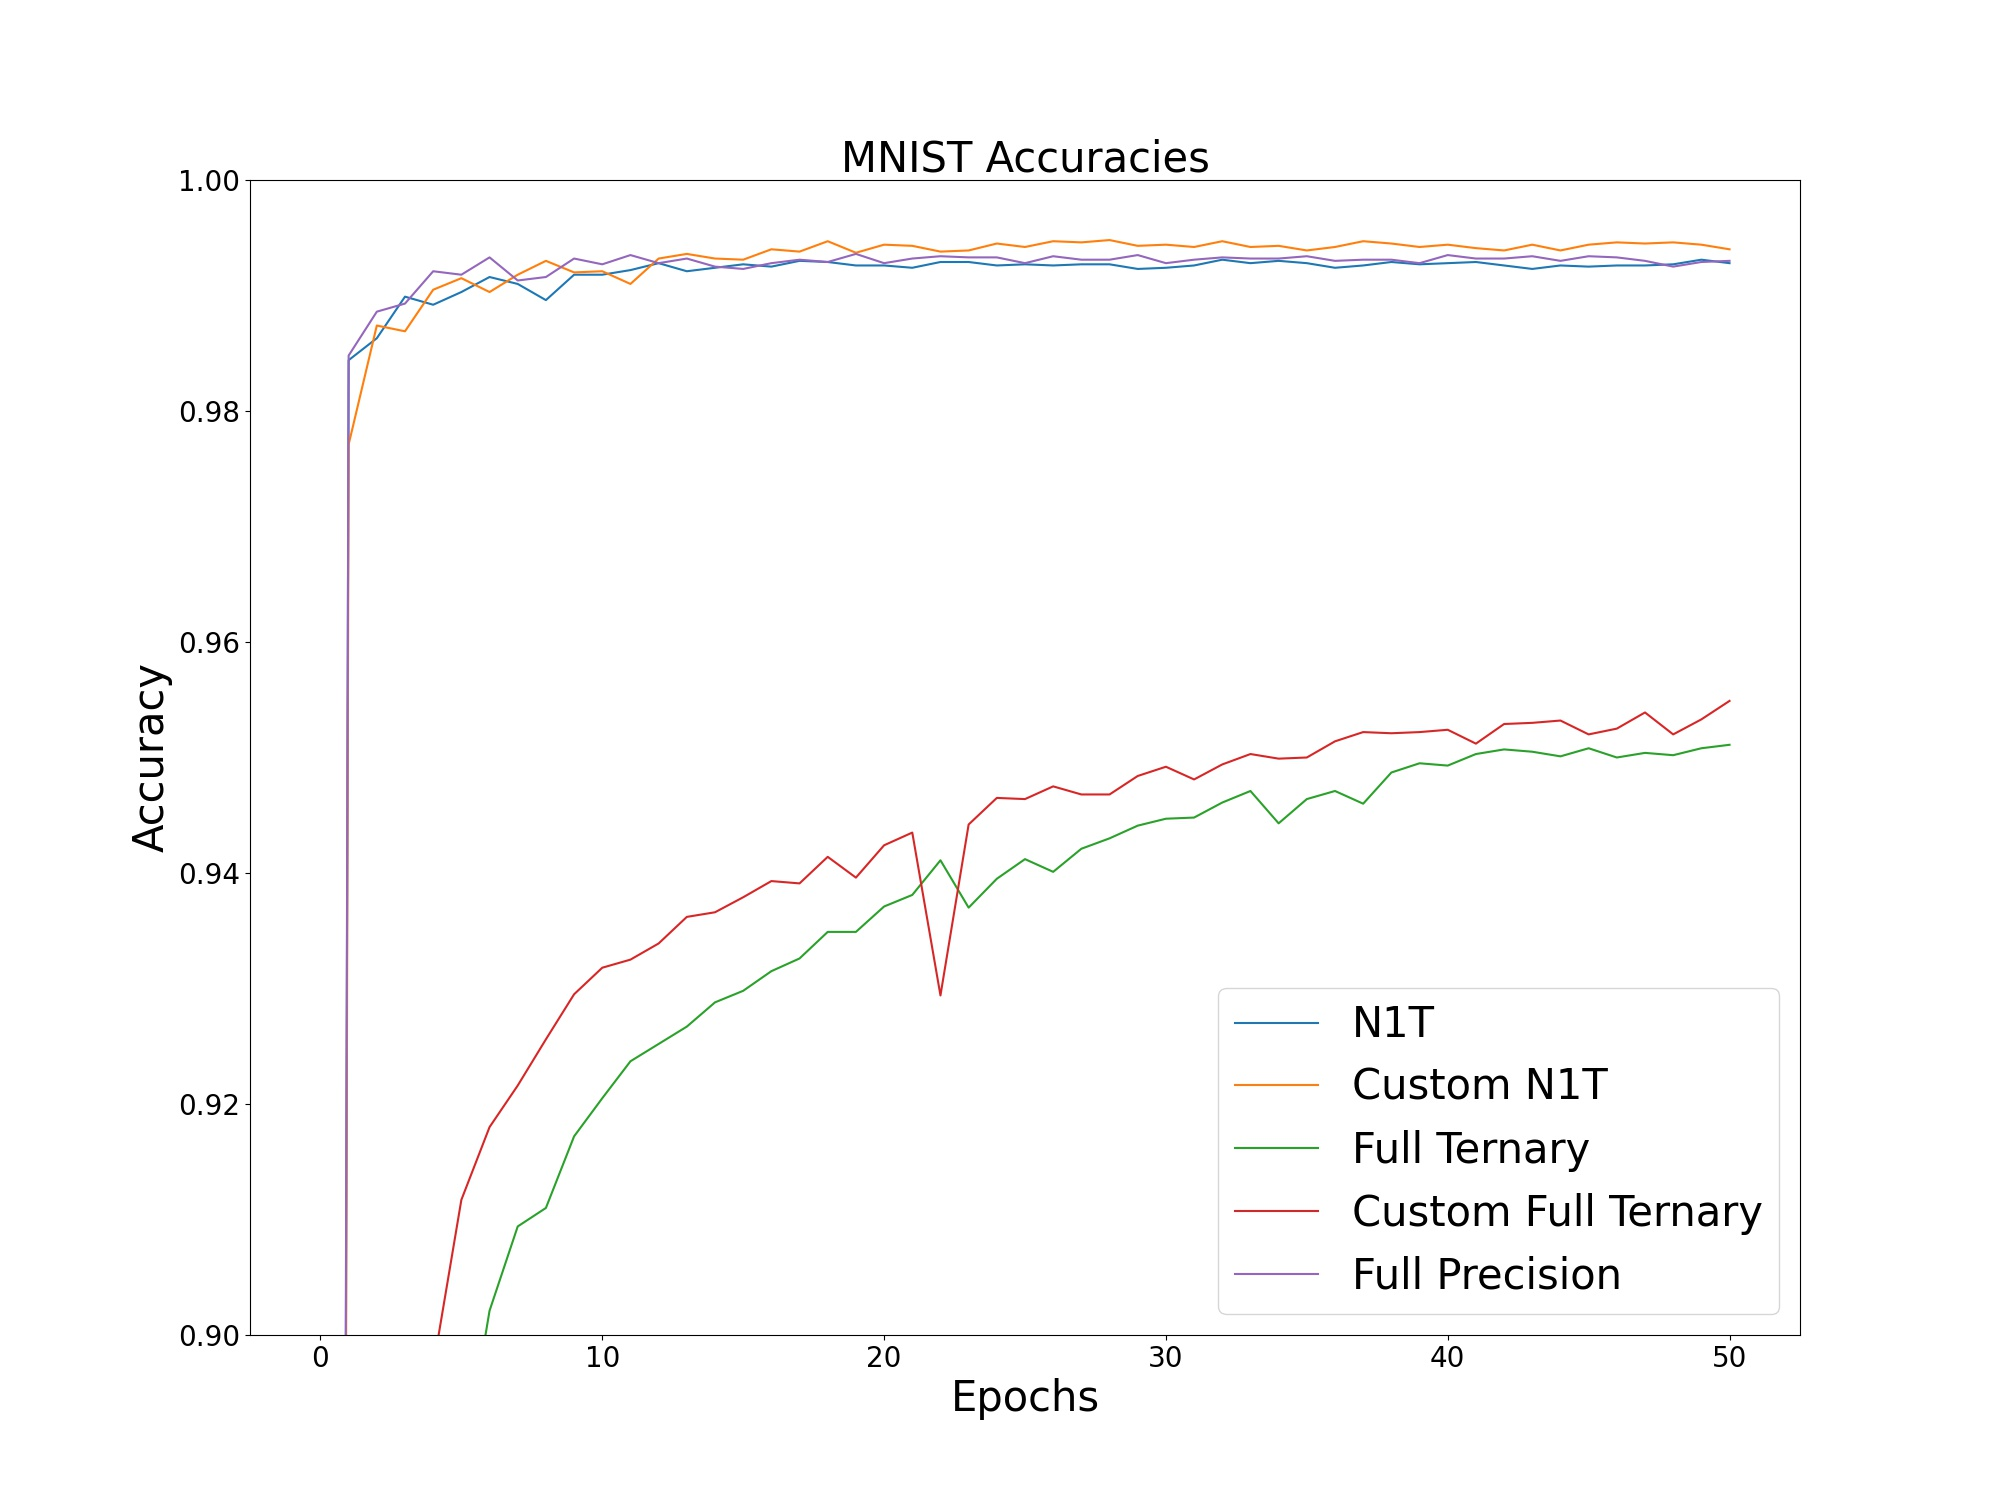
\includegraphics[width=37em]{Results_Images/MNIST_Accuracy_Graph.jpg}
    \caption{LeNet-5 model performance during training on the MNIST dataset. These numbers were recorded after every epoch by running the test portion of the dataset through the network and computing its average accuracy.}
    \label{fig:mnist_accuracy}
\end{figure}

\begin{figure}
    \centering
    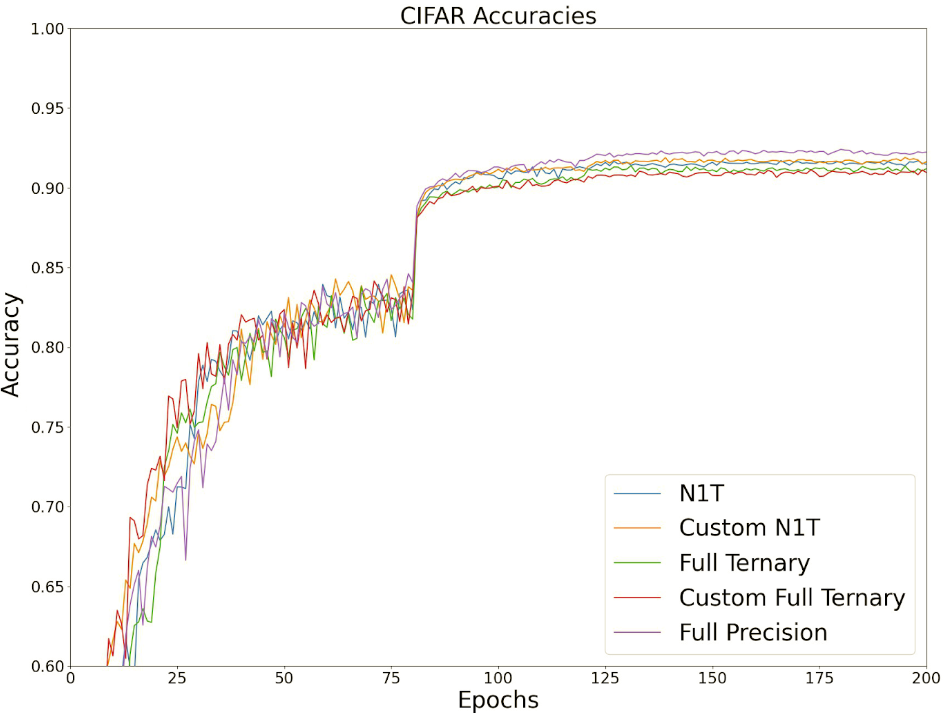
\includegraphics[width=37em]{Results_Images/CIFAR_Accuracy_Graph.jpg}
    \caption{VGG7 model performance during training on the CIFAR-10 dataset. These numbers were recorded in the same fashion as those in Figure \ref{fig:mnist_accuracy}.  Here, the sudden spike in accuracy corresponds to when the learning rate decays, allowing the network to make finer adjustments to itself.}
    \label{fig:cifar_accuracy}
\end{figure}

For our empirical timing experiments, the results we found are listed in Table \ref{tab:res_time_comparison}. There, you can see that our custom filters took just over half the time required by the ternary filters. Interestingly, this is below the estimated ratio of 0.64 from Table \ref{tab:res_comparison}, though there are explanations for this. Firstly, when computing the values for only a single feature, the integral image operations account for approximately 10.5\% of the total operations. When the number of filters is increased, the proportion of the operations belonging to the integral image decreases, so with our example using 32 filters, the integral image accounts for only a scant 0.3\% of the total operations. When we redo the calculations, we find that 32 custom filters, plus their integral image, only uses ~0.57$\times$ the number of operations a ternary layer needs. This number is much more in line with our observations. The remaining difference of 0.04 can be attributed to overheads in the programming language, and slight differences in the efficiency of the data structures used to implement our solution. 

\begin{table}[h]
\centering
    \begin{tabular}{|c | c|} 
        \hline
        \multicolumn{2}{|c|}{MNIST Time Comparison (Seconds)} \\
        \hline
        Custom Filter & ~0.16 \\
        Ternary & ~0.30 \\
        \hline
        \textbf{(Custom Filter / Ternary)} & \textbf{~0.53} \\
        \hline
    \end{tabular}
\caption{The empirical time difference between using standard ternary convolutions and our custom filters. In this, 500 images from the MNIST dataset were used, and the average image processing time was recorded. The final row of this table shows the difference in time between the custom filter and a ternary filter as a ratio.}
\label{tab:res_time_comparison}
\end{table}

\section{Discussion and Future Work}
As shown by our experiments, combining the integral image and Haar-like features from the Viola-Jones framework with a ternary convolutional layer allows for the acceleration of the first layer in a network by significant amounts (provided they are larger than $3\times3$). Since ternary networks are already faster than full precision networks, this increase in performance compounds, potentially allowing for even greater network speeds. Additionally, this improvement comes almost without cost, in terms of accuracy. When compared to other N1T or Full Ternary networks, the accuracy only slightly decreased in the worst examples, and sometimes did the opposite, resulting in better performing networks. 

While admittedly, our efficiency gains only affect the first layer, in many architectures, the first layer contains the largest filters, making it one of the more expensive parts of the network. The Resnet \cite{resnet} and the original YOLO \cite{yolo} networks are popular examples of this, where their first convolutional layer uses numerous $7\times7$ filters. Of these two, YOLO is an especially good candidate for our optimization, as it is meant for real time analysis, so every bit of performance helps. 

\subsection{Limitations}
One major downside to this approach is that, at present, all of our custom filters are created by hand. This is only a minor inconvenience for small networks like LeNet-5 that work on greyscale images, since they require only a handful of custom features, but for colour images on larger networks, it rapidly becomes incredibly time consuming. For example, our VGG7 implementation used 128 filters over three dimensions (the input images were colour), requiring a total of 384 $5 \times 5$ filters to be crafted by hand. An example of these filters is shown in Figure \ref{fig:cifar_custom_filters_128}. This took a significant amount of time, and as the process would need to be repeated whenever the network was retrained with new parameters, new architectures, or a new dataset, it limits our method's usefulness. Additionally, we limited ourselves to only testing our method on the first layer of a network, with good reason: In our VGG7 example, the first layer's output is a stacked matrix of the feature maps output from each filter, leading to a whooping 128 channel input array for the following layer. This is an unacceptably large amount of data to parse by hand, so our proposal is limited to modifying the first layer of the network.

\begin{figure}
    \centering
    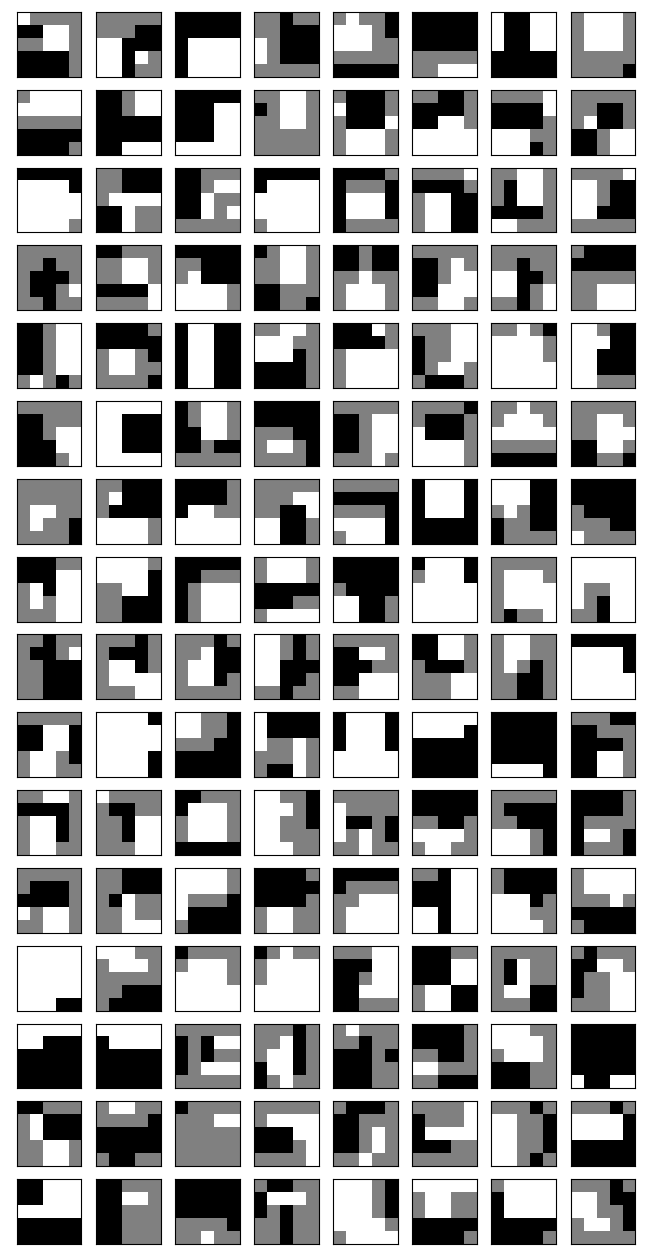
\includegraphics[width=30em]{Methodology_Images/0-custom_filters.png}  % 37
    \caption{The 128 custom filters from one channel (out of three) of the first layer of the VGG7 network. Crafting these by hand was a time consuming task.}
    \label{fig:cifar_custom_filters_128}
\end{figure}


\subsection{Future Work}
These problems are things we would like to solve in future work. We would like to devise an algorithm that would allow us to automatically create optimal custom filters by identifying the four rectangles that would best fit a given ternary weight filter. With this, we could extend our method to work with more complex networks, and additionally, extend our optimizations to the deeper layers of the network, allowing us to bring significant performance gains to larger architectures. Unfortunately, devising such an algorithm would be complex and is beyond the scope of this thesis. 

Additionally, our current empirical run-time experiments were completed using single-threaded code and a representative convolutional layer. This is not ideal, as it deviates from the tools commonly used in the real work. The math tells us our solution should be very efficient, so we would like to reimplement it using parallelism and more performant language, with the intention of comparing it to the convolutional layer implementations from modern machine learning libraries. 


\chapter{Conclusion}
In conclusion, in this thesis, we have presented a method of combining the weight optimizations from ternary weight networks with a set of custom features inspired by the Viola-Jones Object Detection Framework to improve the performance of a network. By replacing the first convolutional layer in a network with a function using a custom set of filters, we are able to reduce the number of operations required to compute the layer's outputs. These filters are composed of four rectangles, labeled as either positive or negative, within the filter space, and when combined with an integral image, allow for more efficient computations of feature values compared to that of a standard convolutional layer. When using our custom filters of shape $5\times5$, the layer only requires $~64\%$ of the operations that a standard convolutional layer would need, and this reduction only increases as the filter sizes get larger. Empirically, we have found that the real-world execution times of these layers behave as theoretically calculated, but also, that their optimizations do not lead to significant drops in accuracy.

During testing, we evaluated our proposed optimization on two different datasets with two different network architectures. The MNIST \cite{mnist} dataset, a collection of greyscale images containing hand-written digits between 0 and 9, was processed with a shallow architecture composed of two convolutional layers and two fully connected layers, called LeNet-5. In this experiment, despite our custom layer representing $~25\%$ of the network, we find that it does not negatively affect the accuracy, while simultaneously allowing for better performance. For the experiments using the CIFAR-10 dataset, a collection of small, RGB images grouped into ten different classes, we used a seven layer deep convolutional network, called VGG-7. In this experiment, which had the more complex task of labeling the images with classifications like `car' or `airplane', again, our optimization resulted in only a very slight drop in accuracy, which is easily justified when the gains in performance are considered.

Our method is not without its flaws, however. Currently, the custom filters must be defined by hand, which becomes very time consuming in more complex network architectures. As such, it is impractical to use beyond the first layer of said networks. We would like to develop an algorithm to automate this in future work, to allow for the use of our optimization in the deeper portions of various networks. This would allow for large performance gains in deep networks, where the number of computations in the first layer are small compared to the number required by the network overall. Despite this, though, we believe our method has merit as is, since it not only provides a performance boost for shallower networks, but can also be combined with the performance gains ternary networks promise over standard, full precision networks, to allow for even faster computations. 


% $2 \times (\textrm{32-C1}) + \textrm{MP2} + 2 \times (\textrm{64-C1}) + \textrm{MP2} + \textrm{512-FC} + \textrm{10-FC}$

%\begin{table}[h]
%\centering
%    \begin{tabular}{|c|c|c|} 
%        \hline
%        & LeNet-5 & VGG7 \\%
%        \hline
%        Optimizer & ADAM & SGD \\
%        Batch Size & 100 & 100 \\
%        Weight Decay & 1e-5 & 1e-4 %\\
%        Learning Rate & 0.001 & 0.1 %\\
%        LR Decay Epochs & N/A & 80, %120 \\
%        Momentum & N/A & 0.9 \\
%        \hline
%    \end{tabular}
%\end{table}


\bibliographystyle{unsrt}
\bibliography{sample}

\end{document}

